\documentclass[landscape,fleqn,7pt]{scrartcl}
\usepackage[left=1cm,right=1cm,top=1cm,bottom=1cm,landscape]{geometry}
\usepackage[utf8]{inputenc}
%%% Packages for LaTeX - programming
%
% Define commands that don't eat spaces.
\usepackage{xspace}
% IfThenElse
\usepackage{ifthen}
%%% Doc: ftp://tug.ctan.org/pub/tex-archive/macros/latex/contrib/oberdiek/ifpdf.sty
% command for testing for pdf-creation
\usepackage{ifpdf} %\ifpdf \else \fi

%%% Internal Commands: ----------------------------------------------
\makeatletter
%
\providecommand{\IfPackageLoaded}[2]{\@ifpackageloaded{#1}{#2}{}}
\providecommand{\IfPackageNotLoaded}[2]{\@ifpackageloaded{#1}{}{#2}}
\providecommand{\IfElsePackageLoaded}[3]{\@ifpackageloaded{#1}{#2}{#3}}
%
\newboolean{chapteravailable}%
\setboolean{chapteravailable}{false}%

\ifcsname chapter\endcsname
  \setboolean{chapteravailable}{true}%
\else
  \setboolean{chapteravailable}{false}%
\fi


\providecommand{\IfChapterDefined}[1]{\ifthenelse{\boolean{chapteravailable}}{#1}{}}%
\providecommand{\IfElseChapterDefined}[2]{\ifthenelse{\boolean{chapteravailable}}{#1}{#2}}%

\providecommand{\IfDefined}[2]{%
\ifcsname #1\endcsname
   #2 %
\else
     % do nothing
\fi
}

\providecommand{\IfElseDefined}[3]{%
\ifcsname #1\endcsname
   #2 %
\else
   #3 %
\fi
}

\providecommand{\IfElseUnDefined}[3]{%
\ifcsname #1\endcsname
   #3 %
\else
   #2 %
\fi
}


%
% Check for 'draft' mode - commands.
\newcommand{\IfNotDraft}[1]{\ifx\@draft\@undefined #1 \fi}
\newcommand{\IfNotDraftElse}[2]{\ifx\@draft\@undefined #1 \else #2 \fi}
\newcommand{\IfDraft}[1]{\ifx\@draft\@undefined \else #1 \fi}
%

% Definde frontmatter, mainmatter and backmatter if not defined
\@ifundefined{frontmatter}{%
   \newcommand{\frontmatter}{%
      %In Roemischen Buchstaben nummerieren (i, ii, iii)
      \pagenumbering{roman}
   }
}{}
\@ifundefined{mainmatter}{%
   % scrpage2 benoetigt den folgenden switch
   % wenn \mainmatter definiert ist.
   \newif\if@mainmatter\@mainmattertrue
   \newcommand{\mainmatter}{%
      % -- Seitennummerierung auf Arabische Zahlen zuruecksetzen (1,2,3)
      \pagenumbering{arabic}%
      \setcounter{page}{1}%
   }
}{}
\@ifundefined{backmatter}{%
   \newcommand{\backmatter}{
      %In Roemischen Buchstaben nummerieren (i, ii, iii)
      \pagenumbering{roman}
   }
}{}

% Pakete speichern die spaeter geladen werden sollen
\newcommand{\LoadPackagesNow}{}
\newcommand{\LoadPackageLater}[1]{%
   \g@addto@macro{\LoadPackagesNow}{%
      \usepackage{#1}%
   }%
}



\makeatother
%%% ----------------------------------------------------------------
\usepackage[ngerman]{varioref}
\usepackage{hyperref}
\usepackage[fleqn]{amsmath}
\usepackage{mathtools} %aligned matrix
\usepackage{multicol}
\usepackage[table]{xcolor}
\usepackage{ragged2e}
%\usepackage{amsfonts}
%\usepackage{amssymb}
%\usepackage{gensymb}
%\usepackage{dsfont}
\usepackage{calc}
%\usepackage[permil]{overpic}
\usepackage{graphicx}
%\graphicspath{{gfx/}}
\usepackage{blindtext}
\usepackage{tikz}
%\usepackage{booktabs}
%\usepackage{multirow}

\usepackage{enumitem}
\usepackage{ltxtable}
\usepackage{float}
\usepackage{subcaption}
\usepackage{tcolorbox}

% section headings and toc
\usepackage{titlesec}
\usepackage{titletoc}

\usepackage[ngerman]{babel}
%% Kommandos fuer Tabellen. Entnommen aus The LateX Companion, tabsatz.ps und diversen Dokus:

%%% ---| Farben fuer Tabellen |-------------------
\IfPackageLoaded{xcolor}{
   \colorlet{tablesubheadcolor}{gray!30}
   \colorlet{tableheadcolor}{gray!25}
   \colorlet{tableblackheadcolor}{black!100}
   \colorlet{tablerowcolor}{gray!10.0}
}
%%% ---------------------------------------------


%%% -| Neue Spaltendefinitionen 'columntypes' |--
%
% Belegte Spaltentypen:
% l - links
% c - zentriert
% r - rechts
% p,m,b  - oben, mittig, unten
% X - tabularx Auto-Spalte

% um Tabellenspalten mit Flattersatz zu setzen, muss \\ vor
% (z.B.) \raggedright geschuetzt werden:
\newcommand{\PreserveBackslash}[1]{\let\temp=\\#1\let\\=\temp}


% Spalten mit Flattersatz und definierte Breite:
% m{} -> mittig
% p{} -> oben
% b{} -> unten
%
% Linksbuendig:
\newcolumntype{v}[1]{>{\PreserveBackslash\RaggedRight\hspace{0pt}}p{#1}}
\newcolumntype{M}[1]{>{\PreserveBackslash\RaggedRight\hspace{0pt}}m{#1}}
% % Rechtsbuendig :
% \newcolumntype{R}[1]{>{\PreserveBackslash\RaggedLeft\hspace{0pt}}m{#1}}
% \newcolumntype{S}[1]{>{\PreserveBackslash\RaggedLeft\hspace{0pt}}p{#1}}
% % Zentriert :
% \newcolumntype{Z}[1]{>{\PreserveBackslash\Centering\hspace{0pt}}m{#1}}
% \newcolumntype{A}[1]{>{\PreserveBackslash\Centering\hspace{0pt}}p{#1}}

\newcolumntype{Y}{>{\PreserveBackslash\RaggedLeft\hspace{0pt}}X}
%%% Spalten fuer Mathematik
%
% serifenlose Matheschrift
\newcolumntype{s}[1]{%
	>{\DC@{.}{,}{#1}\mathsf\bgroup}l%
	<{\egroup\DV@end}%
}

% Tabellenspaltentyp fuer den Kopf: (Farbe + Ausrichtung)
\newcolumntype{H}[1]{>{\columncolor{tableheadcolor}}l}

% aequivalent aus typokurz (fett+grau+links)
% \newcolumntype{H}{>{\fontseries{b}\selectfont%
%     \columncolor[gray]{.8}[6pt][0pt]}l}
%%% --------------------------------------------


%%% ---|Listen in Tabellen |--------------------
\newcommand{\removeindentation}{%
	\leftmargini=\labelsep%
	\advance\leftmargini by \labelsep%
}
%
\makeatletter
\newcommand\tableitemize{
	\@minipagetrue%
	\removeindentation
}
\makeatother
%%% --------------------------------------------

%%% ---|Layout der Tabellen |-------------------

% Neue Umgebung fuer Tabellen:

\newenvironment{Tabelle}[2][c]{%
  \tablestylecommon
  \begin{longtable}[#1]{#2}
  }
  {\end{longtable}%
  \tablerestoresettings
}


% Groesse der Schrift in Tabellen
\newcommand{\tablefontsize}{ \footnotesize}
\newcommand{\tableheadfontsize}{\footnotesize}

% Layout der Tabelle: Ausrichtung, Schrift, Zeilenabstand
\newcommand\tablestylecommon{%
  \renewcommand{\arraystretch}{1.4} % Groessere Abstaende zwischen Zeilen
  \normalfont\normalsize            %
  \sffamily\tablefontsize           % Serifenlose und kleine Schrift
  \centering%                       % Tabelle zentrieren
}

\newcommand{\tablestyle}{
	\tablestylecommon
	%\tablealtcolored
}

% Ruecksetzten der Aenderungen
\newcommand\tablerestoresettings{%
  \renewcommand{\arraystretch}{1}% Abstaende wieder zuruecksetzen
  \normalsize\rmfamily % Schrift wieder zuruecksetzen
}

% Tabellenkopf: Serifenlos+fett+schraeg+Schriftfarbe
\newcommand\tablehead{%
  \tableheadfontsize%
  \sffamily\bfseries%
  %\slshape
  %\color{white}
}

\newcommand\tablesubheadfont{%
  \tableheadfontsize%
  \sffamily\bfseries%
  \slshape
  %\color{white}
}


\newcommand\tableheadcolor{%
	%\rowcolor{tablesubheadcolor}
	%\rowcolor{tableblackheadcolor}
	\rowcolor{tableheadcolor}%
}

\newcommand\tablesubheadcolor{%
	\rowcolor{tablesubheadcolor}
	%\rowcolor{tableblackheadcolor}
}


\newcommand{\tableend}{\arrayrulecolor{black}\hline}

% Tabellenkopf (1=Spaltentyp, 2=Text)
% \newcommand{\tablehead}[2]{
%   \multicolumn{1}{#1@{}}{%
%     \raisebox{.1mm}{% Ausrichtung der Beschriftung
%       #2%
%     }\rule{0pt}{4mm}}% unsichtbare Linie, die die Kopfzeile hoeher macht
% }


\newcommand{\tablesubhead}[2]{%
  \multicolumn{#1}{>{\columncolor{tablesubheadcolor}}l}{\tablesubheadfont #2}%
}

% Tabellenbody (=Inhalt)
\newcommand\tablebody{%
\tablefontsize\sffamily\upshape%
}

\newcommand\tableheadshaded{%
	\rowcolor{tableheadcolor}%
}
\newcommand\tablealtcolored{%
	\rowcolors{1}{tablerowcolor}{white!100}%
}
%%% --------------------------------------------

\newlength{\mylen}
\newlength{\adjusthspace}

\newenvironment{tabularc}[2]
{%
	\setlength\mylen{#2/(#1)-\tabcolsep*2-\arrayrulewidth*(#1+1)/(#1)}%
	%\setlength{\adjusthspace}{((#2-1)/2)*\linewidth}
	%\par\noindent
	%\hspace*{-\the\adjusthspace}
	\begin{tabular}%{#2}%
		{*{#1}{v{\the\mylen}}}%
}
{\end{tabular}\par}



% circled number
\newcommand*\circled[1]{
    \tikz[baseline=(char.base)]{
        \node[shape=circle,draw,inner sep=2pt] (char) {#1};
    }
}
% section heading style
\renewcommand{\thesection}{\protect\circled{\arabic{section}}}
\renewcommand{\thesubsection}{\arabic{section}.\arabic{subsection}}
\titlecontents{section}
[0.0cm]                            % left margin
{\vspace{2em}}                     % above code
{\thecontentslabel}                % numbered format
{\thecontentslabel}                % unnumbered format
{\titlerule*[1pc]{.}\contentspage} % filler-page-format, e.g dots

\setlength{\intextsep}{0mm plus1mm minus1mm}

%\setlength{\abovecaptionskip}{30pt}
\makeatletter
\renewcommand*\env@matrix[1][\arraystretch]{%
    \edef\arraystretch{#1}%
    \hskip -\arraycolsep
    \let\@ifnextchar\new@ifnextchar
    \array{*\c@MaxMatrixCols c}}
\makeatother
\AtBeginEnvironment{bmatrix}{\setlength{\arraycolsep}{1.5pt}}
\AtBeginEnvironment{vmatrix}{\setlength{\arraycolsep}{1.5pt}}
\AtBeginEnvironment{array}{\setlength{\arraycolsep}{1.5pt}}

\author{Stanislav Sokol}
\title{Formelsammlung Regelungstechnik}

\newcommand{\bs}[1]{\boldsymbol{#1}}
\setlength\abovedisplayshortskip{0pt}
\setlength\belowdisplayshortskip{0pt}
\setlength\abovedisplayskip{0pt}
\setlength\belowdisplayskip{0pt}
\abovedisplayskip=5pt plus 3pt minus 5pt 
\abovedisplayshortskip=0pt plus 3pt 
\belowdisplayskip=5pt plus 3pt minus 5pt 
\belowdisplayshortskip=7pt plus 3pt minus 4pt 
\setlength{\mathindent}{0pt}

%\pagenumbering{gobble}
\usepackage{fancyhdr}
\pagestyle{fancy}
\fancyhf{}
\fancyhead[L]{\href{https://github.com/it13104/regelungstechnik-formelsammlung}
                   {github.com/it13104/regelungstechnik-formelsammlung}}
\fancyhead[R]{\thepage}
\begin{document}
\setlength{\columnsep}{1cm}
\begin{multicols}{3}
    \tableofcontents
    \setcounter{section}{1}
\section{Modellierung von dynamischen Systemen}
\begin{tcolorbox}[colback=white!10!white,
                  colframe=blue!50!black,
                  title=KOCHREZEPT: Freischneiden]
    Massen $\{m_1,\hdots,m_n\}$ mit $\{x_1,\hdots,x_m\}$ \\
    Anfangsbedingung: $x_1 = \hdots = x_m = 0$ \\\\
    \begin{minipage}{0.3\textwidth}
        \centering
        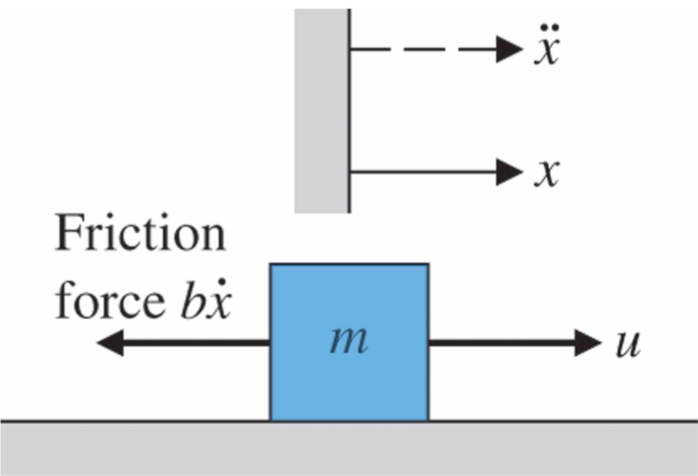
\includegraphics[width=\textwidth]{images/free_body_diagram}
    \end{minipage}
    %\hspace{0.05\textwidth}
    \begin{minipage}{0.65\textwidth}
        \begin{enumerate}
            \item Freischneiden: $\forall{x_i}\forall{x_j}: x_j \neq x_i :$ \\
                $x_j$ ,,festhalten'', \\
                $x_i$ ,,erhöhen'' und Pfeile entgegengesetzt ausrichten, so dass
                \begin{itemize}
                    \item $\forall k: k(x_i - x_j)$
                    \item $\forall b: b(\dot{x}_i - \dot{x}_j)$
                \end{itemize}
            \item Gleichungssystem: \\
                $\sum F = 0 = m_i \ddot{x}_i$ \\
                Vorzeichen aller entgegengesetzten Kräfte sind negativ.
            \item Stabilität: \\
                System ist stabil, sobald mindestens eine $m_i$ unabhängig 
                gedämpft oder das System nur einseitig beschränkt ist.
        \end{enumerate}
    \end{minipage}
\end{tcolorbox}

\begin{tcolorbox}[colback=white!10!white,
                  colframe=gray!50!black,
                  title=Beispiel]
    \begin{minipage}{0.3\textwidth}
        Aufgabe:
        \centering
        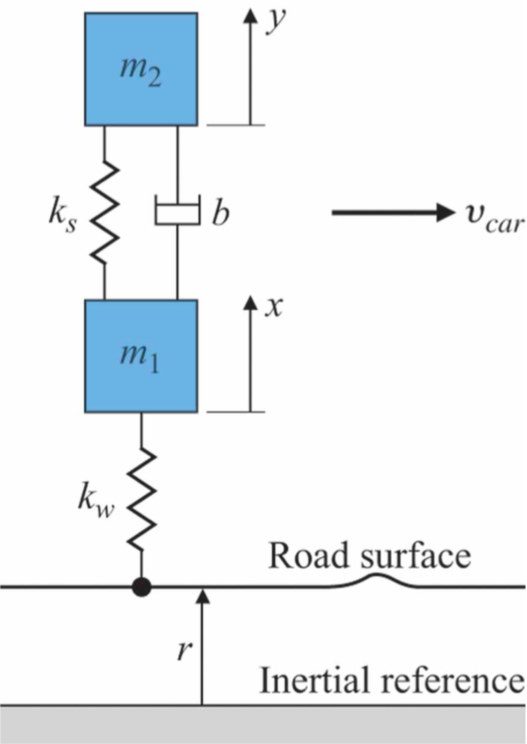
\includegraphics[width=\textwidth]{images/free_body_diag_example1_a}
    \end{minipage}
    \begin{minipage}{0.65\textwidth}
        Freigeschnitten:
        \centering
        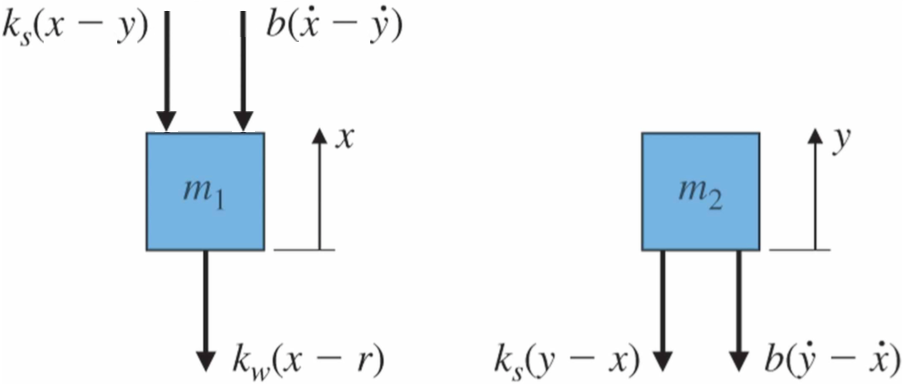
\includegraphics[width=\textwidth]{images/free_body_diag_example1_b}
    \end{minipage}
    Gleichungssystem:
    \begin{equation*}\begin{matrix}
        m_1 \cdot \ddot{x} & = & -k_w(x-r) - k_s(x-y) - b(\dot{x}-\dot{y}) \\
        m_2 \cdot \ddot{y} & = & -k_s(y-x) - b(\dot{y}-\dot{x}) \\\\
        \frac{k_w}{m_1} r & =
            & \ddot{x} + \frac{b}{m_1} \dot{x} + \frac{k_w+k_s}{m_1} x
            - \frac{b}{m_1} \dot{y} - \frac{k_s}{m_1} y \\ 
        0 & = & \ddot{y} + \frac{b}{m_2} \dot{y} + \frac{k_s}{m_2} y
            - \frac{b}{m_2} \dot{x} - \frac{k_s}{m_2} x \\\\
        \frac{k_w}{m_1} R(s) & =
            & \Bigl( s^2 + s\frac{b}{m_1} + \frac{k_w+k_s}{m_1} \Bigr) X(s)
            - \Bigl(s\frac{b}{m_1} + \frac{k_s}{m_1} \Bigr) Y(s) \\ 
        0 & = & \Bigl( s^2 + s\frac{b}{m_2} + \frac{k_s}{m_2} \Bigr) Y(s)
            - \Bigl( s\frac{b}{m_2} + \frac{k_s}{m_2} \Bigr) X(s) \\\\
    \end{matrix}\end{equation*}
\end{tcolorbox}
    \setcounter{section}{2}
\section{Das dynamische Verhalten von Systemen}
\subsection{Blockdiagramme}
\begin{tcolorbox}[colback=white!10!white,colframe=blue!50!black,title=Regeln]
    
    \begin{figure}[H]
        \begin{subfigure}{.3\textwidth}
            \centering
            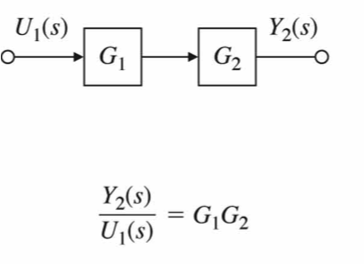
\includegraphics[width=1\textwidth]{images/kettenschaltung}
            \label{fig:kettenschaltung}
            \caption{Kettenschaltung}
        \end{subfigure}%
        \begin{subfigure}{.3\textwidth}
    \centering
    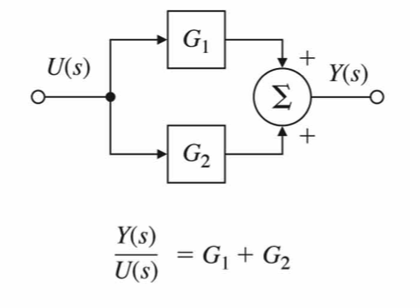
\includegraphics[width=1\textwidth]{images/parallel}
    \caption{Parallelschaltung}
    \label{fig:parallel}
        \end{subfigure}%
            \begin{subfigure}{.3\textwidth}
                \centering
                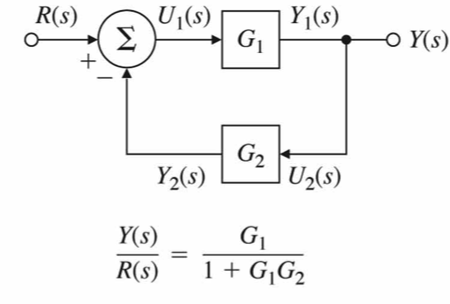
\includegraphics[width=1\textwidth]{images/back}
                \caption{Rückführung}
                \label{fig:back}
            \end{subfigure}%
    \end{figure}
\begin{figure}[H]

            \begin{subfigure}{.5\textwidth}
            \centering
            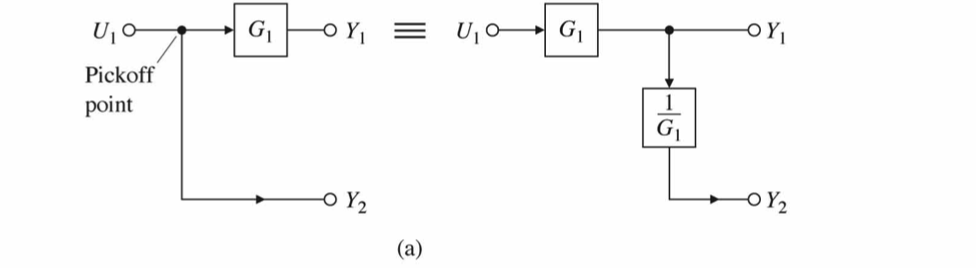
\includegraphics[width=1\textwidth]{images/verschiebung_punkt}
            \caption{Pickoff-Verschiebung}
            \label{fig:pickoff}
            \end{subfigure}%
            \begin{subfigure}{.5\textwidth}
                \centering
                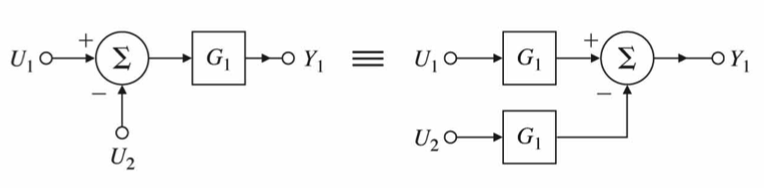
\includegraphics[width=1\textwidth]{images/sum_front}
                \caption{Summationspunkt-Verschiebung}
                \label{fig:sum}
            \end{subfigure}%
            

\end{figure}
\begin{figure}[H]
    \begin{subfigure}{.5\textwidth}
        \centering
        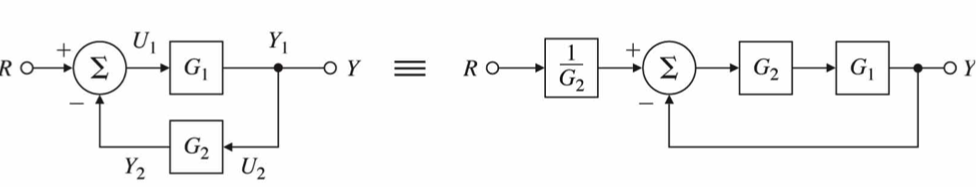
\includegraphics[width=1\textwidth]{images/satz}
        \caption{}
        \label{fig:satz}
    \end{subfigure}%
\end{figure}
\end{tcolorbox}

\begin{tcolorbox}[colback=white!10!white,colframe=gray!50!black,title=Beispiele]
    \begin{figure}[H]
        
        \begin{minipage}{.5\textwidth}
            \centering
            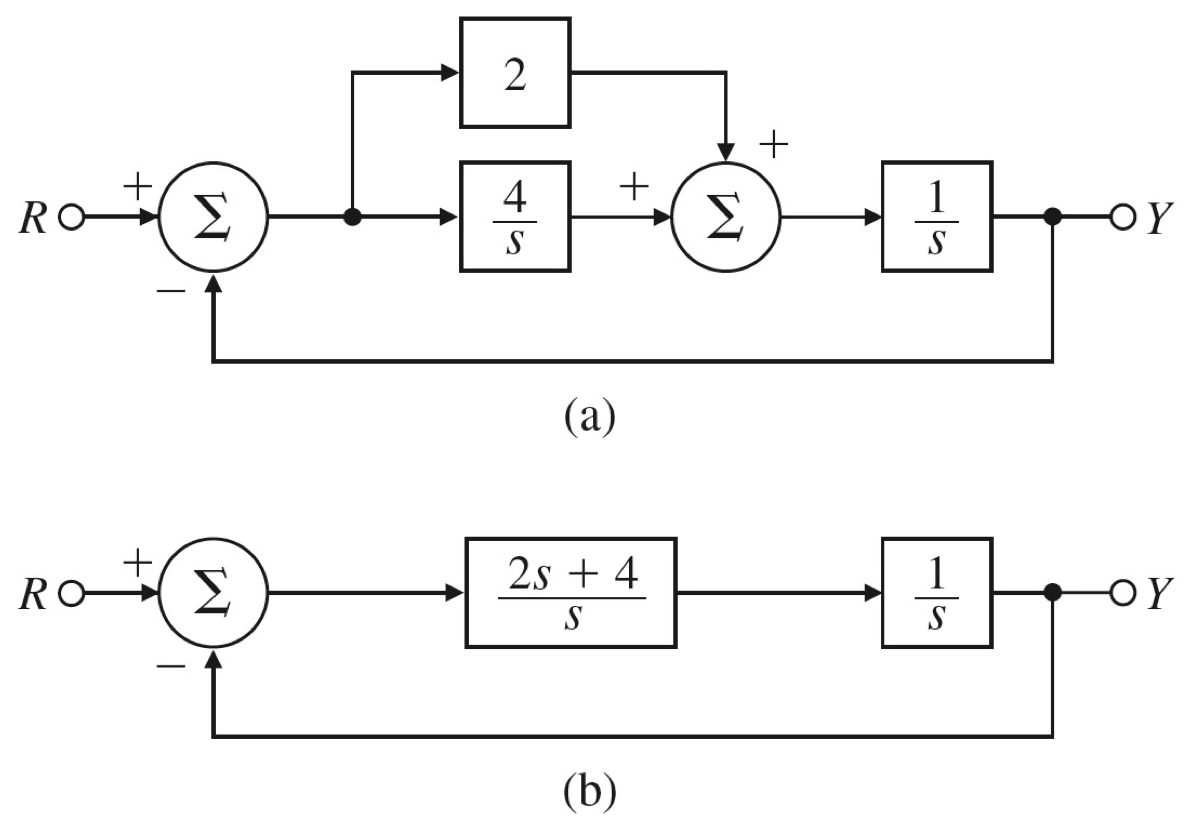
\includegraphics[width=1\textwidth]{images/example_1}
    
        \end{minipage}%
        \begin{minipage}{.5\textwidth}
            \begin{align*}
                T(s) = \frac{\frac{2s+4}{s^2}}{1+\frac{2s+4}{s^2}}
            \end{align*}
        \end{minipage}%
        
        
    \end{figure}
    \begin{figure}[H]
    \noindent\rule[0.2ex]{\linewidth}{1pt}
    
        \begin{minipage}{.5\textwidth}
            \centering
            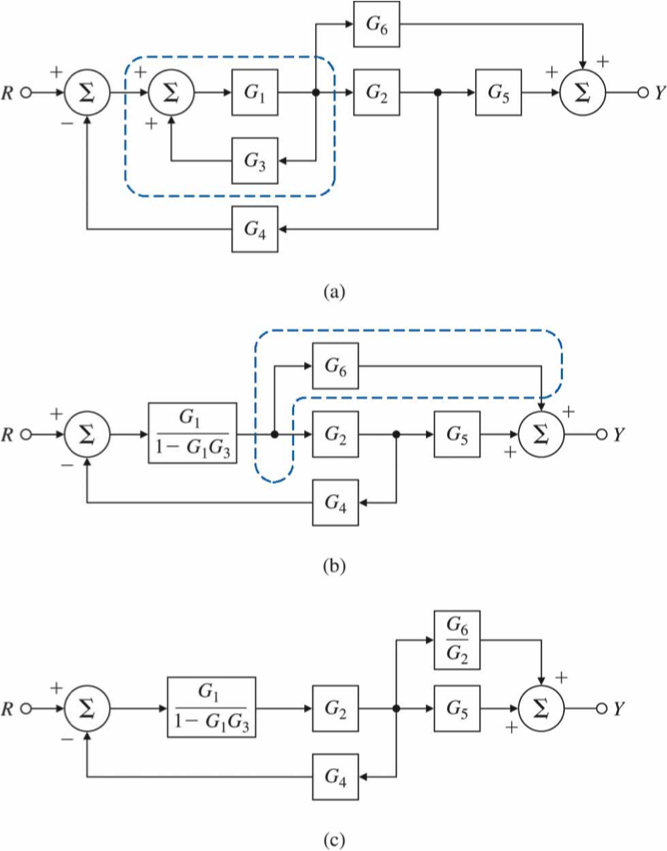
\includegraphics[width=1\textwidth]{images/example_2}
            
        \end{minipage}%
        \begin{minipage}{.5\textwidth}
            \begin{align*}
            &T(s) = \frac{\frac{G_1G_2}{1-G_1G_3}}{1+\frac{G_1G_2G_4}{1-G_1G_3}}\cdot\\& \cdot(G_5+\frac{G_6}{G_2})\\
            &= \frac{G_1G_2G_5+G_1G_6}{1-G_1G_3+G_1G_2G_4}
            \end{align*}
        \end{minipage}%
        
        
    \end{figure}

\end{tcolorbox}

\subsection{Laplace-Transformation}
Wenn nichts anderes gegeben gilt für Anfangsbedingungen $y(0) = \dot{y(0)} =  \ldots = 0$ .

\subsection{Partialbruchzerlegung}
\begin{tcolorbox}[colback=white!10!white,colframe=blue!50!black,title=Regeln]
    \begin{align*}
        &\frac{A}{x-x_1}&\text{Einfache Nullstelle}\\
        &\frac{A_1}{x-x_1}+ \ldots + \frac{A_m}{(x-x_1)^m }&\text{m-fache Nullstelle}\\
        &\frac{Ax+B}{x^2+ax+b} &\text{quadratisch (komplex) Nst}\\
        &\frac{Ax+B}{x^2+ax+b}+ \ldots + \frac{A_mx+B_m}{x^2+ax+b} &\text{m-fach quadratisch Nst}\\
    \end{align*}
\end{tcolorbox}



    \setcounter{section}{3}
\section{Frequenzgang und Polstellenlage}
\begin{tcolorbox}[colback=white!10!white,colframe=green!30!black,title=PT$_2$ - Glied] 
    \begin{figure}[H]
        \begin{minipage}{.3\textwidth}
            \centering
            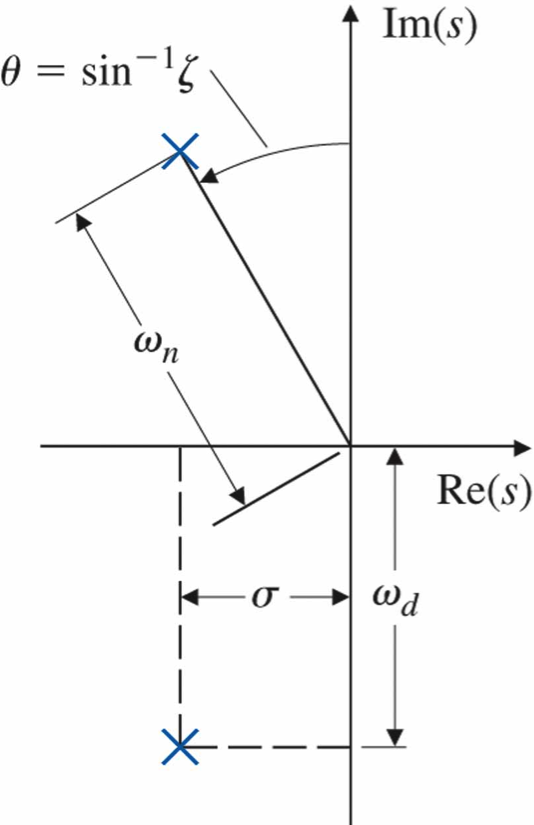
\includegraphics[width=1\textwidth]{content/img/winkel}
        \end{minipage}%
        \hspace{1cm}
        \begin{minipage}{.6\textwidth}
            Instabilität beginnt in der rechten Halbebene. 
            
            Für die  \textbf{Dämpfung} gilt, je kleiner der Winkel $\theta$, desto kleiner ist die Dämpfung: \begin{align*}
                \theta = \arcsin{\zeta}
            \end{align*}
        \end{minipage}%
        
    \end{figure}
    \textbf{Charakteristische Gleichung:} $s^2+2*\zeta*\omega_n*s+\omega_n^2$
\end{tcolorbox}

\begin{tcolorbox}[colback=white!10!white,colframe=green!30!black,title=Auswirkung der NST und Polenlage] 
    \begin{figure}[H]    
            \centering
            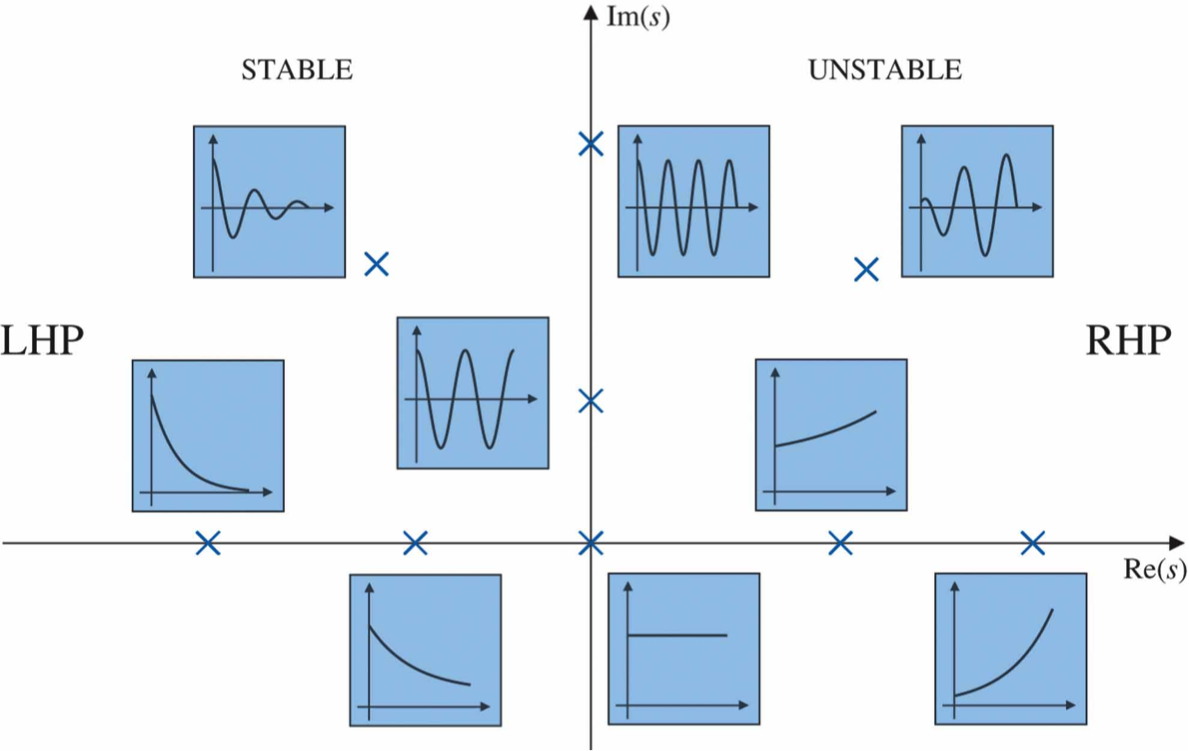
\includegraphics[width=1\textwidth]{content/img/lageAntwort}
    \end{figure}
\tcblower
    \textbf{Polstelle (reell + komplexes Polpaar)}
    \begin{table}[H]
        \centering
        \begin{tabular}{ccc}
            \hline Re & Im & Auswirkung \\ 
            \hline $<$ 0 & = 0 & stabil - keine Schwingung \\ 
            \hline $>$ 0  & =0 & instabil - keine Schwingung \\ 
            \hline $=0$ & =0 & instabil - keine Schwingung \\ 
            \hline\hline $< 0$ & $\not =$ & stabil - Schwingung \\ 
            \hline $> 0$  &  $\not =$ & instabil - Schwingung \\ 
            \hline = 0  & $\not =$ & Dauerschwingung \\ 
            \hline 
        \end{tabular} 
    \end{table}
    \textbf{Nullstelle:}
    \begin{table}[H]
        \centering
        \begin{tabular}{p{2cm}p{3cm}}
            \hline $< = 0 $ & minimalphasiges System (evtl. Überschwung) \\ 
            \hline $> = 0 $ & nichtminimalphasiges System (Systemantwort erst entgegen der Sprunganregung) \\ 
            \hline $= 0 $ & $lim_{t\rightarrow\infty}y(t)\rightarrow 0$ \\ 
            \hline 
        \end{tabular} 
    \end{table}
\end{tcolorbox}
\begin{tcolorbox}[colback=white!10!white,colframe=green!30!black,title=Kenngrößen] 
    \begin{figure}[H]
        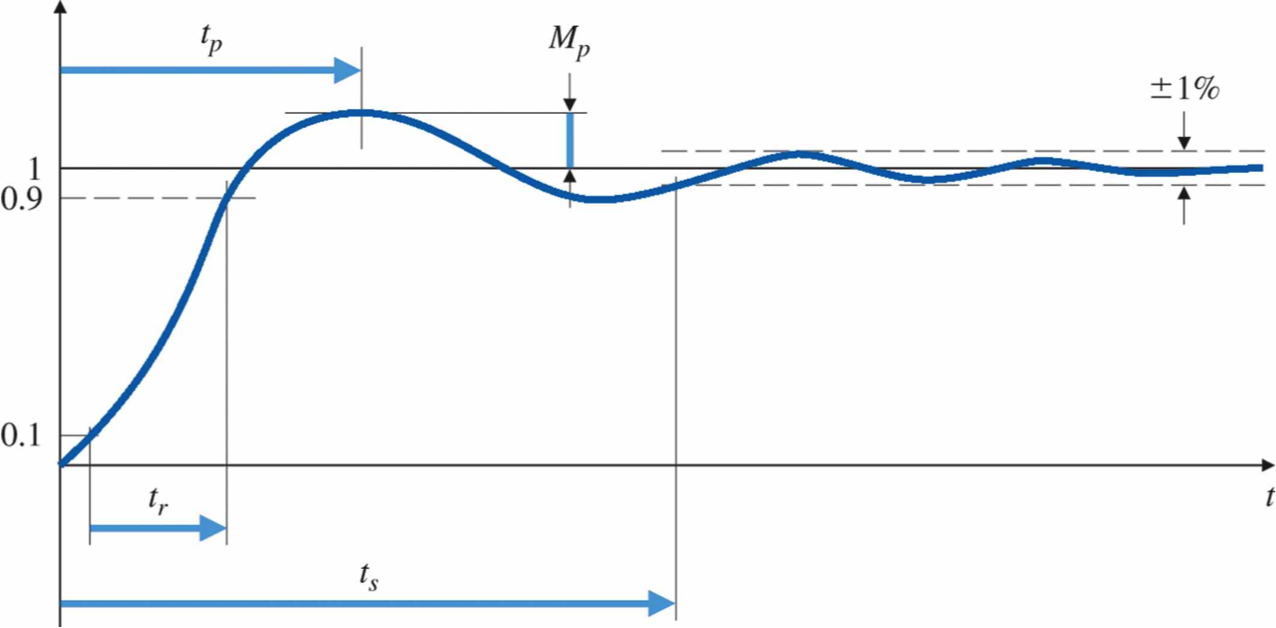
\includegraphics[width=1\linewidth]{content/img/numb}
    \end{figure}
\begin{minipage}{.45\textwidth}
        Steigzeit (0,1 - 0,9):
    \begin{align*}
        t_r &\approx \frac{1,8}{\omega_n} 
    \end{align*}
\end{minipage}
\begin{minipage}{.45\textwidth}
 Einschwingzeit (Abklang auf) $\pm 1\%$
 \begin{align*}
 t_s  &= \frac{4,6}{\zeta\omega_n} = \frac{4,6}{\sigma}
 \end{align*}
\end{minipage}
\begin{minipage}{.45\textwidth}
 Überschwingweite:
 \begin{align*}
 M_p = e^{\frac{-\pi \zeta}{\sqrt{1-\zeta^2}}} \\ 0 \leq \zeta \leq 1
 \end{align*}
\end{minipage}
\begin{minipage}{.45\textwidth}
 Anstiegszeit:
 \begin{align*}
 t_p &= \frac{\pi}{\omega_n \sqrt{1-\zeta^2}} =\frac{\pi}{\omega_d}
 \end{align*}
\end{minipage}    
\begin{minipage}{.45\textwidth}
    Gedämpfte Kreisfrequenz:
    \begin{align*}
        \omega_d = \omega_n*\sqrt{1-\zeta^2}
    \end{align*}
\end{minipage}
\begin{minipage}{.45\textwidth}
    Ungedämpft zu gedämpft
    \begin{align*}
    \omega_n^2 = \sigma^2+\omega_d^2
    \end{align*}
\end{minipage}
    Dämpfung $\zeta = \sqrt{\frac{\ln(M_p)^2}{\pi^2+\ln(M_p)^2}}$
\end{tcolorbox}


    \setcounter{section}{5}
\section{Stabilität von linearen Systemen}
\begin{tcolorbox}[colback=white!10!white,colframe=green!30!black,title=Stabilität] 
Alle Pole der Übertragungsfunktion müssen in der LHE sein. \textbf{Steuerung} stabilisiert nicht. 
\textbf{Regelung:}

    \begin{figure}[H]
        \centering
        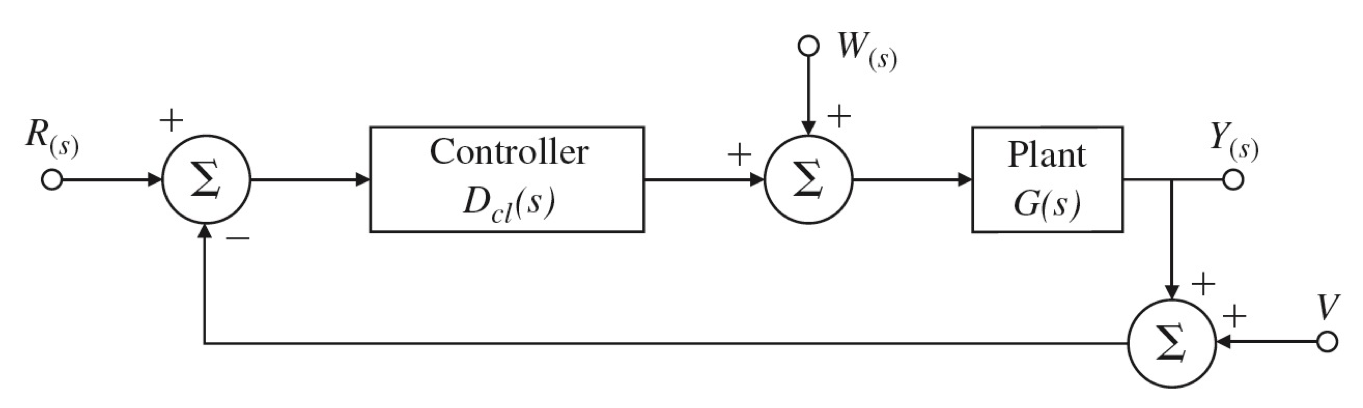
\includegraphics[width=.7\textwidth]{images/regler}
\end{figure}
    \begin{align*}
    &G(s) = \frac{b(s)}{a(s)}  && D_{OL} = \frac{c(s)}{d(s)}
    &1+ G D_{CL} = 0\\ 
    &1 + \frac{bc}{ad} = 0  &&
    a(s)d(s) + b(s)c(s) = 0 
    \end{align*}
Die Regelung reduziert die Auswirkung von Störung um $1+ AK$
\end{tcolorbox}

%ROUTH-Criterion
\subsection{Routh-Stabilitätskritetium}
\begin{tcolorbox}[colback=white!10!white,colframe=green!30!black,title=Routh Kriterium] 
    Gibt Aussage darüber, ob alle Pole des charakteristischen Polynoms $P(s)$ in der LHE liegen:
    \begin{align*}
        P(s) = s^n + a_1s^{n-1}+a_2s^{n-2}+\ldots + a_{n-1}s+a_n
    \end{align*}
    Es muss gelten $a_i > 0$ für $\forall i \in \mathrm{N}$
    \begin{align*}
        \begin{matrix}[0.6]
        n & s^n & 1 & a_2 & a_4 & \ldots \\
        n-1 & s^{n-1} & a_1 & a_3 & a_5 & \ldots \\
        n-2 & s^{n-2} & b_1 & b_2 & b_3 & \ldots \\        
        n-3 & s^{n-3} & c_1 & c_2 & c_3 & \ldots \\
        \vdots & \vdots & \vdots & \vdots & \vdots  \\
        2 & s^2 & * & *  \\
        1 & s^1 & * \\
        0 & s^0 & \ldots
        \end{matrix}
    \end{align*}
    Die Koeffizienten werden folgendermaßen errechnet:
    \begin{align*}
        & b_1 = -\frac{\begin{vmatrix}
            1 & a_2 \\ a_1 & a_3
            \end{vmatrix}}{a_1} = \frac{a_1a_2-a_3}{a_1} & c_1 = -\frac{\begin{vmatrix}
            a_1 & a_3 \\ b_1 & b_2
            \end{vmatrix}}{b_1} = \frac{b_1a_3-a_1b_2}{b_1}\\
        & b_2 = -\frac{\begin{vmatrix}
            1 & a_4 \\ a_1 & a_5
            \end{vmatrix}}{a_1} = \frac{a_1a_4-a_5}{a_1} & c_2 = -\frac{\begin{vmatrix}
            a_1 & a_5 \\ b_1 & b_3
            \end{vmatrix}}{b_1} = \frac{b_1a_5-a_1b_3}{b_1}\\
        & b_3 = -\frac{\begin{vmatrix}
            1 & a_6 \\ a_1 & a_7
            \end{vmatrix}}{a_1} = \frac{a_1a_6-a_7}{a_1} & c_3 = -\frac{\begin{vmatrix}
            a_1 & a_7 \\ b_1 & b_4
            \end{vmatrix}}{b_1} = \frac{b_1a_7-a_1b_4}{b_1}
    \end{align*}
    
    \begin{itemize}
        \item Alle Elemente der ersten Spalte positiv $\Rightarrow$ Wurzeln in der offenen LHE                
        \item $\#$-Wurzeln  in der geschlossenen RHE   = $\#$-Vorzeichenwechsel 
        \item Wenn das erste Element einer Zeile null ist, setze $\epsilon > 0$. Stabilitätskriterium für $\epsilon \rightarrow 0_+$
    \end{itemize}
\end{tcolorbox}


\begin{tcolorbox}[colback=white!10!white,colframe=green!30!black,title=Sensitivität] 
    Sensitivität beschreibt die Reaktion des Systems auf Änderung im Parameter
    \begin{align*}
        & S_{A}^{T_{CL}} = \frac{A}{T_{CL}}\frac{d T_{CL}}{dA}
        & |S_{G}^{T_{CL}}| = \frac{1}{1+G(i\omega_0)D(i\omega_0)}
        \end{align*}
    \begin{align*}
        &T_{CL} -\text{ Closed-Loop Übertragungsfunktion} & A - \text{Parameter}
    \end{align*}
\end{tcolorbox}
%CLM-Criterion
\subsection{CLM-Stabilitätskriterium}
\begin{tcolorbox}[colback=white!10!white,colframe=green!30!black,title=CLM Kriterium] 
    \textbf{Annahme:}
    $m$-Wurzeln in RHE  und $n-m$-Wurzeln ($n \leq m$)
    
    Charakteristische Gleichung:
    \begin{align*}
        P(s) = a_0 + a_1s + a_2s^2 + \ldots + a_n s^n = 0 
    \end{align*}
    Einsetzen $s = j\omega$. 
    Das System ist dann asymptotisch stabil, wenn
    \begin{enumerate}
        \item die Ortskurve $P(j\omega)$  für $0 \leq \omega \leq \infty$ die Quadranten abwechselnd durchläuft (sich die Nullstellen des Real und Imaginärteils von $P(j\omega) = U(\omega)+iV(\omega)$ abwechseln.) 
        \item Real- und Imaginärteil zusammen $n$ (Grad der Gleichung) reelle Nullstellen im Bereich $0 \leq \omega \leq \infty$ besitzen 
    \end{enumerate} 
    
    
    
    
    \tcblower
    
    \textbf{Beispiel:}
    \begin{align*}
        &P(s) = 2 + 5s +7s^2 +8s^3 +4s^4 +s^5\\
        &P(j\omega) = 2 + 5j\omega + 7(j\omega)^2 +8 (j\omega)^3 + 4 (j\omega)^4 + (j\omega)^5\\
        &2-7\omega^2 +4\omega^4 + j (5\omega - 8\omega^3 +\omega^5)\\
        &U(\omega) + jV(\omega)
    \end{align*}
    Realteil hat die Nullstellen:
    \begin{align*}
        &2-7\omega^2 +4\omega^4 = 0 \\
        &\omega_1^2 = 0,36 & \omega_2^2= 1,39
    \end{align*}
        Imaginärteil hat die Nullstellen:
        \begin{align*}
        &5\omega - 8\omega^3 +\omega^5= 0 \\
        &\omega3 = 0  & \omega_4^2= 0,68 & & \omega_5^2= 7,32 
        \end{align*}
        
        Insgesamt sind $n=5$ reelle Nullstellen mit $\omega_i >= 0$. Diese wechseln sich jeweils ab, damit ist das System asymptotisch stabil. $\omega_3 < \omega_1 < \omega_4 < \omega_2 < \omega_5$ Siehe Grafik:
        \begin{figure}[H]
\centering
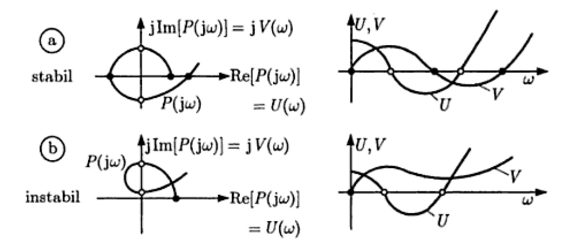
\includegraphics[width=0.7\linewidth]{images/clm}
\label{fig:clm}
\end{figure}

        
\end{tcolorbox}


    \setcounter{section}{7}
\section{Wurzelortskurve}
\begin{tcolorbox}[colback=white!10!white,colframe=blue!50!white,title=Konstruktionsregeln]
    $n$ - Anzahl der Pole ($p_i$)\hspace{1cm}
    $m$ - Anzahl der NST ($z_i$)
    \tcblower  %makes a horizontal line
    \textbf{Regel 1:}\\
    $n-m$ Zweige gehen zu den  Asymptoten\\
    $m$ Zweige enden in den NSTs\\

    \textbf{Regel 2:}\\
        Ein Punkt ist auf WOK, wenn die Summe der Pole und NST rechts vom Punkt ungerade ist (0 ist ungerade) (Nur Pole und NST auf der reellen Achse)\\
        
    \textbf{Regel 3:}\\
    Asymptoten schneiden sich im Schwerpunkt $\alpha$ und haben Winkel $\Phi_l$, $l =1,\dots,n-m$
    \begin{align*}
        \Phi_l &= \frac{180^\circ}{n-m}+\frac{360^\circ(l-1)}{n-m}\\
        \alpha &=    \frac{\sum p_i - \sum z_i}{n-m}
    \end{align*}
        \textbf{Regel 4:}\\
        Beachte Laufindex: $l=1,\dots,q$\\
        Austrittswinkel  der Zweige $q$-Facher Pol. $\Phi_i$- Winkel aus der Sicht der Polstelle. $\Psi_i$ - Winkel aus der Sicht der Nullstelle.
        \begin{align*}
            \Phi_{l,Beginn} &= \frac{1}{q}\left (\sum\Psi_i-\sum_{i\not= l}\Phi_i-180^\circ-360^\circ(l-1)\right )
        \end{align*}
        Eintrittswinkel in die $q$-fachen Nullstellen:
        \begin{align*}
            \Psi_{l,End} &= \frac{1}{q}\left (\sum\Phi_i-\sum_{i\not= l}\Psi_i+180^\circ+360^\circ(l-1)\right )
        \end{align*}
        \textbf{Regel 5:}\\
        Austrittswinkel aus einem Verzweigungspunkt ($q$-facher Pol):
        \begin{align*}
            \Psi_l = \frac{180^\circ}{q}+360^\circ\frac{l-1}{q}
        \end{align*}
        \textbf{Regel 6:}\\
        Verzweigungspunkte Pole (Nullstellen):
        \begin{align*}
            \sum_{i=1}^{m}\frac{1}{s-z_i}-\sum_{i=1}^{n}\frac{1}{s-p_i} =0
        \end{align*}
        \textbf{Charakteristische Gleichung:}
        \begin{align*}
            1+ K*L(s) = 0
        \end{align*}
        
        \textbf{Berechnung von $\bs{K}$:}
        
        Das gesuchte $s$ in die Gleichung einsetzen und die Gleichung lösen
        \begin{align*}
            K = -\frac{\prod_{i}(s-p_i)}{\prod_{i}(s-z_i)}
        \end{align*}
\end{tcolorbox}

    \setcounter{section}{6}
\section{Bode-Diagramm}
\begin{tcolorbox}[colback=white!10!white,
                  colframe=blue!50!white,
                  title=Konstruktionsregeln Bode-Diagramm]
    \textbf{Amplitudengang:}
    \begin{align*}
        &G(s) = c\cdot s^r\cdot \underbrace{G_1(s) \cdot G_2(s)\cdot \ldots \cdot G_k(s)}_{G^*(s)}\cdot e^{-T_ts}\\
        &G_i(s)  = (s+n_i)  \text{ reelle Nullstelle}\\
    \end{align*}
    \begin{enumerate}
        \item Eckfrequenzen aufsteigend sortieren
        \item niedrigste Frequenz ist die Startfrequenz $\omega_1$
        \item Startamplitude:\\ $A_{\text{dB}}(\omega_{\text{min}}) = 20 \log_{10}(|c\cdot G^{*}(0)|\cdot \omega_{\text{min}}^r)$
        \item Asymptote links vom Startpunkt:\\
        $r\cdot20 \frac{\text{dB}}{\text{Dekade}}$
        \item Wenn zwischen benachbarten Eckfreuqenzen 1 Dekade liegt $\Rightarrow$ Absenkung(POL)/Erhöhung(NST) um  $n*3$dB über dem jeweiligen Knickpunkt
        \item Jede Eckfrequenz verändert die Steigung folgendermaßen
            \begin{description}[leftmargin=14em,style=nextline]
                \item[$G_i = (s+n_i)$] $+20\frac{\text{dB}}{\text{Dekade}}
                                        ~~~ \omega_i=\left|n_i\right|$
                \item[$G_i = \frac{1}{(s+p_i)}$] $-20\frac{\text{dB}}{\text{Dekade}}
                                                  ~~~ \omega_i=\left|p_i\right|$
                \item[$G_i = (s^2 + 2D_im_is+m_i^2)$] $+40\frac{\text{dB}}{\text{Dekade}}
                                                       ~~~ \omega_i=\left|m_i\right|$
                \item[$G_i = \frac{1}{(s^2 + 2D_ip_is+p_i^2)}$] $-40\frac{\text{dB}}{\text{Dekade}}
                                                                 ~~~ \omega_i=\left|p_i\right|$
            \end{description}
        \item Jeder Term der Form $s^2 + 2D_im_is+m_i^2$ liefert einen Peak  am entsprechenden $\omega_i$. Eine Nullstelle unterhalb der Asymptote - eine Polstelle oberhalb der Asymptote.\\
        $(\pm)20\log(\frac{1}{2*D_i})$
    \end{enumerate}
    Exakter Wert: $A_{dB}(\omega) = 20 \cdot \log_{10} \left(G(\omega)\right)$
    \tcblower
    \textbf{Phasengang:}
    \begin{enumerate}
        \item Bestimme Startfrequenz\\
        $\varphi(0) = \begin{cases}
    r\cdot 90^\circ &\mbox{wenn } c\cdot G^*(0)>0\\
    -180^\circ+r\cdot 90^\circ & \mbox{wenn } c\cdot G^*(0)<0
        \end{cases} $
        \item an jeder Eckfrequenz springt die Phase:
        \begin{description}[leftmargin=14em,style=nextline]
            \item[$G_i = (s+n_i)$] $+90^\circ\cdot\mbox{sign}(n_i)$
            \item[$G_i = \frac{1}{(s+p_i)}$] $-90^\circ\cdot\mbox{sign}(p_i)$
            \item[$G_i = (s^2 + 2D_im_is+m_i^2)$] $+180^\circ\cdot\mbox{sign}(D_im_i)$
            \item[$G_i = \frac{1}{(s^2 + 2D_iq_is+q_i^2)}$] $-180^\circ\cdot\mbox{sign}(D_iq_i)$
        \end{description}
        \item Wenn $2D_iq_is = 0 \rightarrow$ ungedämpftes Polpaar $\rightarrow\mbox{sign}(0) = \pm 1$ (kann gewählt werden)
    \end{enumerate}
    Exakter Wert: \\
        $\varphi(\omega) = \sum\limits_{j} \arctan\left(-\frac{b}{a}\right)
        : \forall G_j(i\omega) \in G^* : \begin{cases}
            b + ai \\
            \frac{1}{a + bi}
        \end{cases}$
\end{tcolorbox}

\begin{tcolorbox}[colback=white!10!white,colframe=green!30!black,title=Phasenminimumsystem]
\textbf{Phasenminimumsystem} ist dann gegeben, wenn die Übertragungsfunktion
\begin{itemize}
    \item keinen Totzeitfaktor enthält
    \item G(s) hat Pole und Nullstelle nur in LHE
\end{itemize}
\end{tcolorbox}

    \setcounter{section}{8}
\section{Nyquist-Diagramm (Stabilität)}
\begin{tcolorbox}[colback=white!10!white,
                  colframe=blue!50!white,
                  title=Konstruktionsregeln Nyquist-Diagramm]
    \begin{enumerate}
    \item Betrag und Phase für mehrere Punkte aus dem Amplitudengang und 
        Phasengang des Bode-Diagramms ablesen. 
    \item Die Länge des Zeigers $10^{\frac{A_{dB}(\omega)}{20}}$ zum Nyquist-Plot ist der 
        Wert im Amplitudengang.
    \item Der Winkel des Zeigers ist $\varphi(\omega)$
    \item Für $\omega = 0^{\circ}$ bis $\omega = \infty$
    \item Instabil, wenn der Nyquist-Plot die $-1$ umschließt.
\end{enumerate}
\begin{figure}[H]
    \begin{subfigure}{0.5\linewidth}
        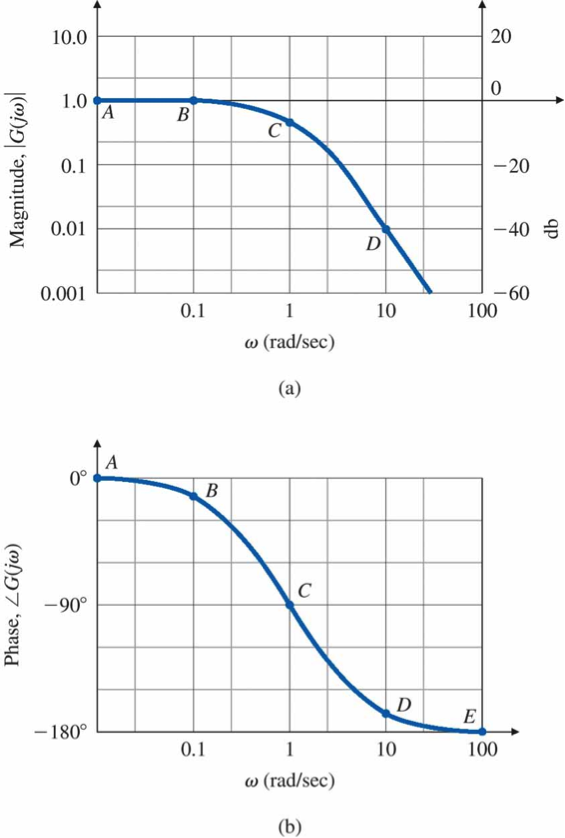
\includegraphics[width=\linewidth]{images/nyquist2}
    \end{subfigure}
    \begin{minipage}{0.45\linewidth}
        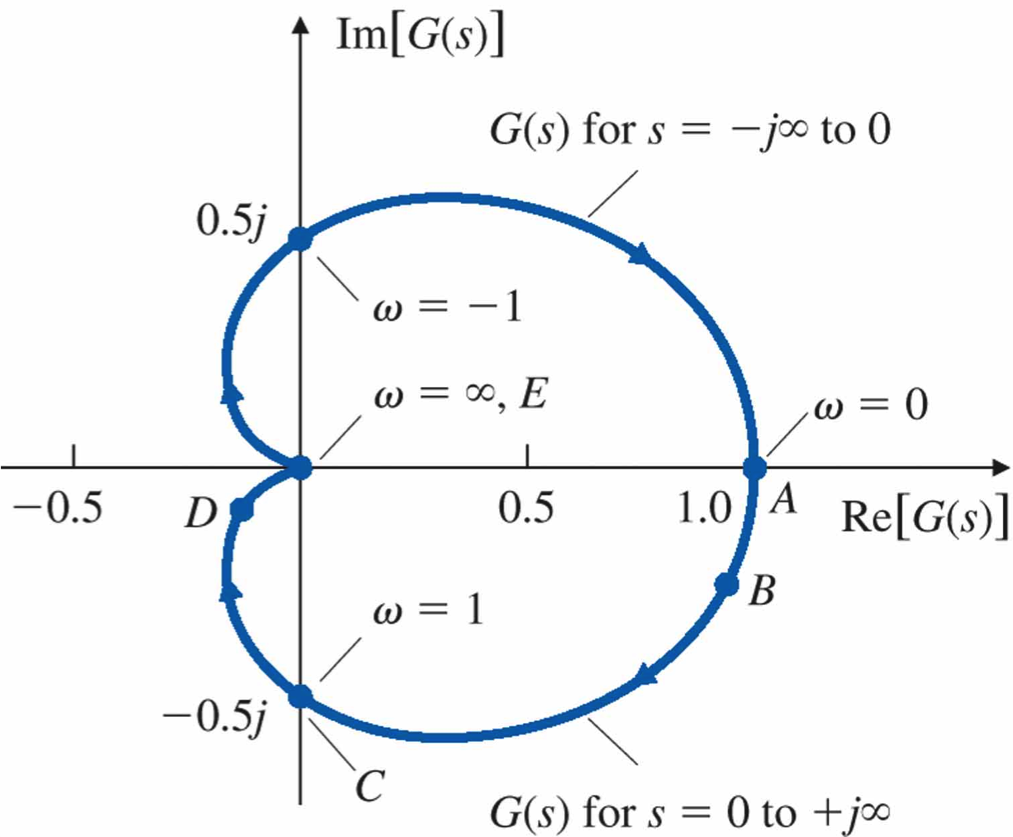
\includegraphics[width=\linewidth]{images/nyquist3}
    \end{minipage}
\end{figure}
\end{tcolorbox}

\begin{tcolorbox}[colback=white!10!white,
    colframe=green!30!black,
    title=Nyquist]
    \begin{figure}[H]
        \begin{subfigure}{0.5\linewidth}
            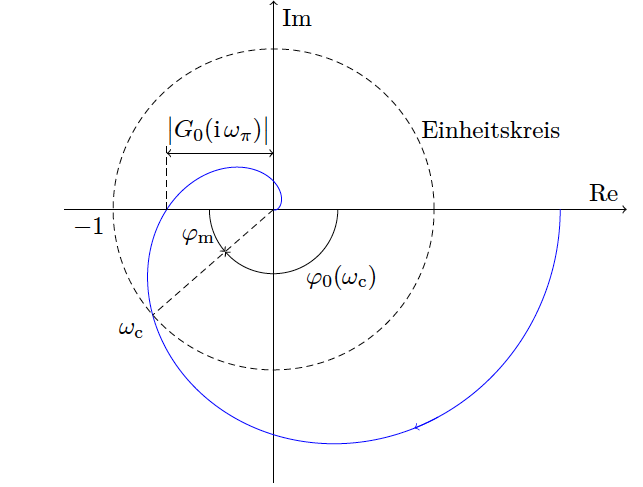
\includegraphics[width=\linewidth]{images/nyquist}
            \label{fig:nyquist}
        \end{subfigure}
        \begin{minipage}{0.45\linewidth}
            Amplituden-/ Betragsreserve 
            \begin{align*}
            &G_m = \frac{1}{|G_0(i\omega_\pi)|}\\
            & \omega_\pi = -180^{\circ}
            \end{align*}
            Phasenreserve ($\omega_c$ ist im Bode Diagramm, da wo Amplitudengang $0$dB schneidet):
            \begin{align*}
            &\phi_m = \pi + \phi(\omega_c)
            \end{align*}
        \end{minipage}
        Übliche Werte sind $G_m = 2,5 \ldots  10$ und $\phi_m = 30^{\circ} \dots 60^{\circ}  $. 
        
        Zur Stabilitätsanalyse kann man prüfen $|G_0(i\omega_\pi)| $ größer oder kleiner als 1 ist. 
    \end{figure}
    \tcblower
    \begin{figure}[H]\centering\begin{tikzpicture}
        \node(b2n) at (0,0) [
            inner sep=0pt,outer sep=0pt,anchor=north west
        ] {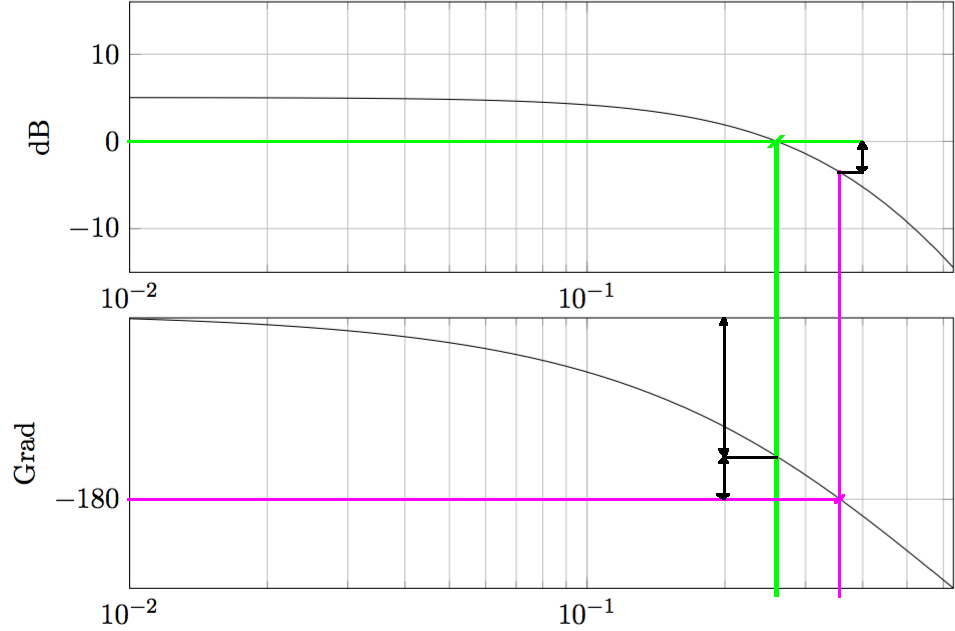
\includegraphics[width=\textwidth]{images/bode2nyquist1}};
        \node(omega-c) at (b2n.south) [
            inner sep=0pt,outer sep=0pt,anchor=south,
            yshift=0.01\textwidth,
            xshift=0.32\textwidth,
        ] {$\omega_c$};
        \node(phi-0) at (b2n.center) [
            inner sep=0pt,outer sep=0pt,anchor=north,
            yshift=-0.05\textwidth,
            xshift=0.23\textwidth,
        ] {$\varphi_0$};
        \node(phi-m) at (phi-0.south) [
            inner sep=0pt,outer sep=0pt,anchor=north,
            yshift=-0.085\textwidth,
        ] {$\varphi_m$};
        \node(omega-pi) at (b2n.south) [
            inner sep=0pt,outer sep=0pt,anchor=south,
            yshift=0.01\textwidth,
            xshift=0.39\textwidth,
        ] {$\omega_\pi$};
        \node(G-0) at (b2n.center) [
            inner sep=0pt,outer sep=0pt,anchor=north,
            yshift=0.22\textwidth,
            xshift=0.42\textwidth,
        ] {$G_0\left(i\omega_\pi\right)$};
        \end{tikzpicture}\end{figure}
    Mit $\varphi_m = \pi + \varphi_0\left(\omega_c\right)$ und
    $G_m = \frac{1}{\left|G_0\left(i\omega_\pi\right)\right|}$
\end{tcolorbox}

\begin{tcolorbox}[colback=white!10!white,colframe=red!60!black,title=Berechnung Betragsreserve aus G(s)]
     Gegeben ist eine Übertragungsfunktion:
     \begin{align*}
        &G(s) = \frac{10}{s^3+11s^2+11s+10}
     \end{align*}
     $j\omega$-Einsetzen  - und auf die untere Form bringen:
     
     Umformen auf
     \begin{align*}
         G(j\omega) &= \frac{10}{\text{Re} + j\omega \text{Im}} = \\
         &=\frac{10}{(-11\omega^2+10)+i\omega (11-\omega^2)}\\
         \tan(-\pi) &= 0 = \frac{\omega_{\pi}(11-\omega_{\pi}^2)}{ \omega_{\pi}^2 +10}\\
     \omega_{\pi} &= \sqrt{11}\\
     G(i\omega_{\pi}) &= \frac{10}{-111}  = 20,9 \text{dB}
     \end{align*}
\end{tcolorbox}

    \setcounter{section}{9}
\section{Zustandsraumdarstellung}

\begin{tcolorbox}[colback=white!10!white,colframe=blue!70!black,title=Übertragungsfunktion aus Zustandsraumdarstellung]
    \begin{tcolorbox}[colback=white!10!white,colframe=gray!70!black,title=Matrixinversion]
        
        \begin{align*}
            G(s) = \frac{Y(s)}{U(s)} &= \boldsymbol{C}(s\boldsymbol{I}-\boldsymbol{A})^{-1}\boldsymbol{B}+D
        \end{align*}
    \end{tcolorbox}
    
    \begin{tcolorbox}[colback=white!10!white,colframe=gray!70!black,title=Verallgemeinerte Systemmatrix]
            Rosenbrockmatrix aufstellen:
            \begin{align*}
                \boldsymbol{P}(s) &= 
            \left[\begin{array}{c|c}
            s\boldsymbol{I}-\boldsymbol{A} & \boldsymbol{B} \\\hline
            -\boldsymbol{C} & D 
            \end{array}\right]    
            \end{align*}
        Übertragungsfunktion:
        \begin{align*}
            G(s) &= \frac{\boldsymbol{C} adj(s\boldsymbol{I}-\boldsymbol{A})\boldsymbol{B}+D|s\boldsymbol{I}-\boldsymbol{A}|}{|s\boldsymbol{I}-\boldsymbol{A}|}\\
            &= \frac{|\boldsymbol{P}(s)|}{|s\boldsymbol{I}-\boldsymbol{A}|}
        \end{align*}
            
    \end{tcolorbox}
    
\end{tcolorbox}

    \setcounter{section}{10}
\section{Kanonische Formen}
\begin{tcolorbox}[colback=white!10!white,colframe=green!60!black,title=Definition + Umrechnung]
\begin{minipage}{.45\textwidth}
    Allgemeine Darstellung:
    \begin{align*}
    \dot{\bs{x}} &= \bs{Fx} + \bs{G}u\\
    y &= \bs{Hx} +Ju
    \end{align*}
\end{minipage}
\begin{minipage}{.45\textwidth}
Darstellung in Normalform:
\begin{align*}
\dot{\bs{x}} &= \bs{Ax} + \bs{B}u\\
y &= \bs{Cx} +Du
\end{align*}
\end{minipage}
\tcblower
\begin{minipage}{.45\textwidth}
    \begin{align*}
    \bs{A} &= \bs{T}^{-1}\bs{F}\bs{T}\\
 \bs{B} &= \bs{T}^{-1}\bs{G}
    \end{align*}
\end{minipage}
\begin{minipage}{.45\textwidth}
    \begin{align*}
        \dot{\bs{x}} &= \bs{Fx} + \bs{G}u\\
        y &= \bs{Hx} +Ju
    \end{align*}
\end{minipage}

\end{tcolorbox}



\begin{tcolorbox}[colback=white!10!white,colframe=blue!70!black,title=KOCHREZEPT: Regelungsnormalform]
    \textbf{Definition:}
    \begin{align}
        Y(s) &= \frac{b(s)}{a(s)} U(s) \\ & = \frac{b_1s^{n-1}+\cdots+b_{n-1}s+b_n}{s^n+a_1s^{n-1}+\cdots + a_{n-1}s+a_n} U(s)\label{eq:uebertragung}\\
        \dot{\bs{x}} &= 
        \begin{bmatrix}
            0 & 1 & \cdots & 0\\
            \vdots & \vdots & \ddots & \vdots \\
            0&0&\cdots&1\\
            -a_n&-a_{n-1}&\cdots&-a_1
        \end{bmatrix}\bs{x}+ 
        \begin{bmatrix}
            0 \\ \vdots \\0\\1
        \end{bmatrix} u \\
        y&= \begin{bmatrix}
            b_n & b_{n-1} & \cdots & b_1
        \end{bmatrix} \bs{x}
    \end{align}


    \tcblower
    Bilde die Inverse $\bs{\mathcal{C}}^{-1}$ von:
    \begin{align*}
        \bs{\mathcal{C}} = \begin{bmatrix}
            G & FG & \cdots & F^{n-1}G
        \end{bmatrix}
    \end{align*}
    Nehme letzte Zeile $\bs{t}_1^T$ von $\bs{\mathcal{C}}^{-1}$ 
    \begin{align*}
        \begin{bmatrix}
            0 & 0 & \cdots & 1
        \end{bmatrix} \bs{\mathcal{C}}^{-1}
    \end{align*}
    Stelle inverse der Transformationsmatrix $\bs{T}$ auf:
    \begin{align*}
        \bs{T}^{-1} &= \left[\begin{array}{l}
        \bs{t}_1^T \\
        \bs{t}_1^T \bs{F}\\
        \bs{t}_1^T \bs{F}^2\\
        \vdots\\
        \bs{t}_1^T \bs{F}^{n-1}
        \end{array}\right]
    \end{align*}
    
    \begin{tcolorbox}[colback=white!10!white,colframe=blue!70!black,title=Umrechnungsvorschrift Zustandsform]
        \begin{align*}
            \bs{B} = \begin{bmatrix}
            0\\ 0\\ \vdots \\1
            \end{bmatrix} \hspace{0.5cm}
            &
            \bs{A} = \bs{T}^{-1}\bs{FT} &
            \bs{C} = \bs{HT}
        \end{align*}
    \end{tcolorbox}
    
    \begin{tcolorbox}[colback=white!10!white,colframe=gray!70!black,title=Steuerbarkeit]
        Das System heißt \textbf{steuerbar}, wenn $\bs{\mathcal{C}}$ \textbf{nicht singulär} ist. (Es existiert eine Inverse von $\bs{\mathcal{C}}$)
    \end{tcolorbox}
\end{tcolorbox}

 
\begin{tcolorbox}[colback=white!10!white,colframe=blue!70!black,title=KOCHREZEPT: Beobachtungsnormalform]
    \textbf{Definition:}
Aus der Funktion \ref{eq:uebertragung} stellt man die Matrizen auf:
    \begin{align*}
        \dot{\bs{x}} &= 
        \begin{bmatrix}
            0 &  \cdots & 0 &-a_n\\
            1 &\cdots & 0 & -a_{n-1} \\
            \vdots&\ddots&\vdots&\vdots\\
            0&\cdots&1&-a_1
        \end{bmatrix}\bs{x}+ 
        \begin{bmatrix}
            b_n \\ b_{n-1} \\ \vdots \\b_1
        \end{bmatrix} u \\
        y&= \begin{bmatrix}
            0 & \cdots & 0& 1
        \end{bmatrix} \bs{x}
    \end{align*}
    \begin{tcolorbox}[colback=white!10!white,colframe=gray!70!black,title=Umrechnungsregeln]
        \begin{align*}
            \bs{A}_O = \bs{A}_C^T &\hspace{0.3cm} \bs{B}_O = \bs{C}_C^T \\
            \bs{C}_O = \bs{B}_C^T   &\hspace{0.3cm} D_O = D_C
        \end{align*}
    
    \end{tcolorbox}

    \tcblower
    Bilde die Inverse $\bs{\mathcal{O}}^{-1}$ und nehme letzte \textbf{Spalte} $\bs{t}_1$ von $\bs{\mathcal{O}}^{-1}$
        
        \begin{align*}
        \bs{\mathcal{O}} &= 
        \left[\begin{array}{l}
        \bs{H}\\
        \bs{HF}\\
        \vdots\\
        \bs{HF}^{n-1}
        \end{array}\right] \rightarrow \bs{\mathcal{O}}^{-1} &      \bs{t}_1 = \bs{\mathcal{O}}^{-1}     \begin{bmatrix}
        0 \\ 0 \\ \vdots \\ 1
        \end{bmatrix}
        \end{align*}

    Die Transformationsmatrix bilden $\bs{T}$ nach Vorschrift:
    \begin{align*}
    \bs{T} &= \left[\begin{array}{llll}
    \bs{t}_1 & \bs{Ft}_1 & \dots & \bs{F}^{n-1}\bs{t}_1
    \end{array}\right]
    \end{align*}
    
    \begin{tcolorbox}[colback=white!10!white,colframe=blue!70!black,title=Umrechnungsvorschrift in Beobachtungsnormalform]
        \begin{align*}
        \bs{C} = \begin{bmatrix}
        0 & 0& \dots &1
        \end{bmatrix} 
        \\
         \bs{A} = \bs{T}^{-1}\bs{FT} 
        \\
            \bs{B} = \bs{T}^{-1}\bs{G}
        \end{align*}
    \end{tcolorbox}
    
    \begin{tcolorbox}[colback=white!10!white,colframe=gray!70!black,title=Beobachtbarkeit]
        Das System heißt \textbf{beobachtbar}, wenn $\bs{\mathcal{O}}$ \textbf{nicht singulär} ist. (Es existiert eine Inverse von $\bs{\mathcal{O}}$)
    \end{tcolorbox}
\end{tcolorbox}

\begin{tcolorbox}[colback=white!10!white,colframe=blue!70!black,title=KOCHREZEPT: Modalform]
    Partialbruchzerlegung der Übertragungsfunktion $\Rightarrow$ Modus
\\

\begin{enumerate}
    \item Alle Pole sind \underline{reell} und \underline{einfach}:
    \begin{align*}
    G(s) = \frac{b_1}{s-p_1}+ \cdots +\frac{b_n}{s-p_n}
    \end{align*}
    \begin{align*}
    \dot{\bs{x}} = 
    \begin{bmatrix}[1]
    p_1 & 0 &\cdots & 0 \\
    0&p_2 &\cdots & 0  \\
    \vdots&\vdots&\ddots&\vdots\\
    0&0&\cdots&p_n
    \end{bmatrix}\bs{x}+ 
    \begin{bmatrix}
    1\\ 1 \\ \vdots \\1
    \end{bmatrix} u     
    \end{align*}
    \begin{align*}
    y= \begin{bmatrix}
    b_1 & b_2&\cdots &b_n
    \end{bmatrix} \bs{x}
    \end{align*}
    \textbf{Jordanform -  wenn die Nullstellen nicht reell sind:}
    \item Komplexes Polpaar $\Rightarrow$ Partialbruch der Art.
    Blockmatrizen für das Polpaar werden an entsprechender Stelle eingefügt
    \begin{align*}
        \frac{b_{i+1}s+b_i}{s^2+a_is+a_{i+1}}
    \end{align*}
    \begin{align*}
        \dot{\bs{x}} = \begin{bmatrix}
            0 & 1\\
            -a_{i+1} & -a_i
        \end{bmatrix}\bs{x} + \begin{bmatrix}
        0\\1
        \end{bmatrix}u & & \bs{y} = \begin{bmatrix}
        b_i & b_{i+1}
        \end{bmatrix}\bs{x}
    \end{align*}
    
    \item Ein $m$-facher Pol $\frac{b}{(s-p)^m}$
    \begin{align*}
        \dot{\bs{x}} = \begin{bmatrix}
            p&1&\cdots&0&0\\
            0&p&\cdots&0&0\\
            \vdots&\vdots&\ddots&\vdots&\vdots\\
            0&0&\cdots&p&1\\
            0&0&\cdots&0&p
        \end{bmatrix}\bs{x} + \begin{bmatrix}
        0\\0\\\vdots\\0\\1
        \end{bmatrix} u &&\bs{y} = \begin{bmatrix}
        b&0&\cdots&0&0
        \end{bmatrix}\bs{x}
    \end{align*}
    
\end{enumerate}

    \tcblower
    Zum erstellen der Modalform:
    \begin{align}
        \text{Eigenwerte } \lambda_i \text{ von } \bs{F} berechnen\\
        \text{Eigenvektoren von } \bs{F} \text{ bilden } \bs{T}
    \end{align}
        \begin{tcolorbox}[colback=white!10!white,colframe=blue!70!black,title=Umrechnungsvorschrift in Modalform]
            \begin{align*}
            \bs{A} = \text{diag}\{\lambda_1,\dots,\lambda_n\} &
             \\
            \bs{B} = \bs{T}^{-1}\bs{G} 
            &
            \hspace{1cm}\bs{C} = \bs{HT}
            \end{align*}
        \end{tcolorbox}

    \begin{tcolorbox}[colback=white!10!white,colframe=gray!70!black,title=Aussagen]
        Für $\bs{B}$ - wenn $b_i = 0$ $\Rightarrow x_i$ \textbf{nicht steuerbar}
        
        Für $\bs{C}$ - wenn $c_i = 0$ $\Rightarrow x_i$ \textbf{nicht beobachtbar}
        
        
        
    \end{tcolorbox}        
        
    
\end{tcolorbox}

\paragraph{Aufgabe:}
Stellen Sie folgende Übertragungsfunktion in Jordannormalform dar:
\begin{align*}
    G(s) &=  \frac{2s+4}{s^2(s^2+2s+4)} = \frac{1}{s^2} - \frac{1}{s^2+2s+4}
\end{align*}
\textbf{Lösung:}
\begin{align*}
    \begin{bmatrix}
    \dot{x}_1\\\dot{x}_2\\\dot{x}_3\\\dot{x}_4
        \end{bmatrix} = \left[\begin{array}{cc|cc}
        0&1&0&0\\
        0&0&0&0\\\hline
        0&0&0&1\\
        0&0&-4&-2\\
        \end{array}\right]\begin{bmatrix}
        x_1\\x_2\\x_3\\x_4
        \end{bmatrix} + \begin{bmatrix}
            0\\1\\0\\1
        \end{bmatrix}u && y = \begin{bmatrix}
        1 &0&-1&0
        \end{bmatrix}x
\end{align*}


    \setcounter{section}{12}
\section{Regelung im Zustandsraum}
\subsection{Regler-Entwurf}
\begin{tcolorbox}[colback=white!10!white,colframe=green!30!black] 

    \begin{enumerate}
        \item     Die Zustandsrückführung ist : $u = -\bs{Kx}$ einsetzen in $\dot{\bs{x}} = \bs{Fx}+\bs{G}u$
        \item $\dot{\bs{x}} = (\bs{F}-\bs{GK})\bs{x}$
        \item Für vorgegebene Pole $s_i$ charakteristische Gleichung aufstellen
        \item $\det (s\bs{I}-\bs{F}+\bs{GK})$ ergibt die charakteristische Gleichung in Abhängigkeit von $\bs{K} = \begin{bmatrix}
        k_1 & \ldots & kn
        \end{bmatrix}$
        \item Koeffizentenvergleich zwischen beiden charakteristischen Gleichungen $\Rightarrow \bs{K}$ 
    \end{enumerate} 
\tcblower
\textbf{System in Regelungsnormalform}
$K$ ist besonders einfach, wenn ein System in RNF vorliegt.
\begin{align*}
    \bs{A}_C-\bs{B}_C\bs{K} = \begin{bmatrix}
    0 & 1& 0&\ldots&0\\     0 & 0& 1&\ldots&0\\
    0 & 0& 0&\ddots&0\\
    0 & 0& 0&\ldots&1\\
    -a_n-k_1 & -a_{n-1}-k_2& &\ldots&-a_{1}-k_n\\
    \end{bmatrix}
\end{align*}
Die charakteristische Gleichung ergibt sich sofort zu:
\begin{align*}
    s^n +(a_1+k_n)s^{n-1}+(a_2+k_{n-1})s^{n-2}+\ldots+(a_n+k_1) =0 
\end{align*}

Man kann direkt den Koeffizientenvergleich machen - Determinantenbildung entfällt.
    
\end{tcolorbox}

\begin{tcolorbox}[colback=white!10!white,colframe=green!30!black,title=Integralregelung]
    Charakteristische Gleichung $0=det(s\bs{I}-\bs{A}_a+\bs{B}_a*\bs{K})$
    Integralregelung  sorgt dafür der Fehler bei Änderung der Streckenparameter Null wird. Das System wir um einen Integralen Teil erweitert.
    \begin{align*}
        \begin{bmatrix}
        \dot{    \bs{x}_I} \\ \dot{    \bs{x}}
        \end{bmatrix} &= \begin{bmatrix}
        0 & \bs{H} \\ 0 & \bs{F}
        \end{bmatrix}\begin{bmatrix}
            \bs{x}_I \\    \bs{x}
        \end{bmatrix}+
        \begin{bmatrix}
        0 \\ \bs{G}
        \end{bmatrix} u - \begin{bmatrix}
        1 \\ 0
        \end{bmatrix}r
    \end{align*}
    mit dem Regler:
    \begin{align*}
        u = -\begin{bmatrix}
         K_1 & \bs{K_0}
        \end{bmatrix} \begin{bmatrix}
            \bs{x}_I \\\bs{x}
        \end{bmatrix} = - \bs{K} \begin{bmatrix}
        \bs{x}_I \\\bs{x}
        \end{bmatrix}
    \end{align*}
    
    \begin{figure}[H]
\centering
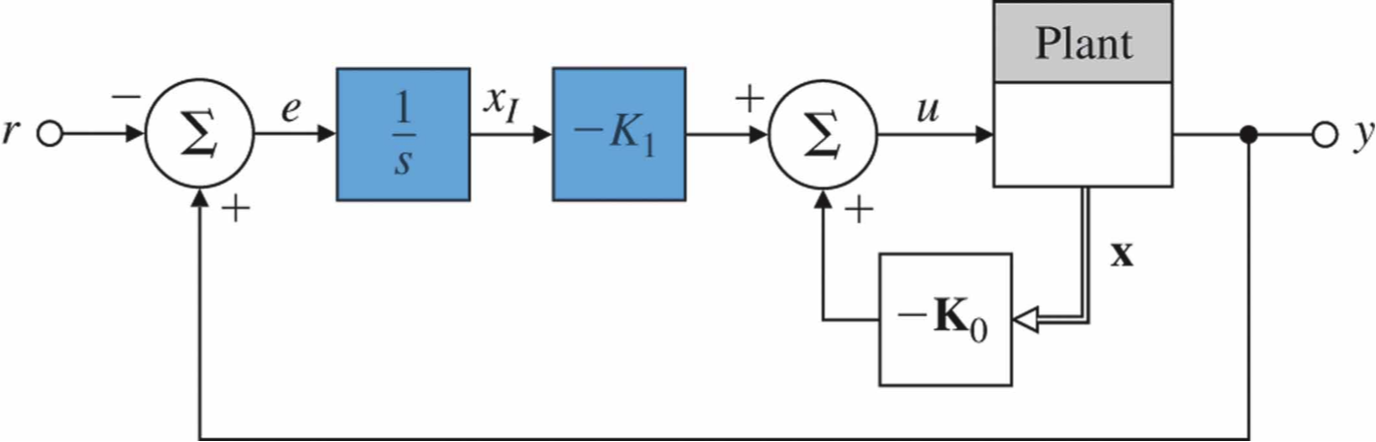
\includegraphics[width=0.7\linewidth]{content/img/integral}

\end{figure}
\tcblower
\textbf{Beispiel:}
Übertragungsfunktion $\frac{Y(s)}{U(s)} = \frac{1}{s+3}$\\
Systembeschreibung $F = -3, G = 1, H = 1$

Gewünscht Pole bei $s=-5$ + Integralanteil \\$\Rightarrow a_C(s) = s^2+10s+25$

Die erweiterte Systembeschreibung ergibt sich zu:
\begin{align*}
        \begin{bmatrix}
        \dot{    \bs{x}_I} \\ \dot{    \bs{x}}
        \end{bmatrix} = \begin{bmatrix}
            0 & 1\\ 0 & -3
        \end{bmatrix} \begin{bmatrix}
        \bs{x}_I \\\bs{x}
        \end{bmatrix} + \begin{bmatrix}
        0 \\1
        \end{bmatrix}u - \begin{bmatrix}
        1\\0
        \end{bmatrix}r
\end{align*}
Die Rückführmatrix 
\begin{align*}
    &\det\left( s\bs{I} - \begin{bmatrix}
    0 & 1\\ 0 & -3
    \end{bmatrix}+ \begin{bmatrix}
    0 \\1
    \end{bmatrix}\bs{K}\right) \overset{!}{=} s^2 +10s +25\\
    &\bs{K} = \begin{bmatrix}
        K_1 & K_2
    \end{bmatrix} = \begin{bmatrix}
    25 & 7
    \end{bmatrix}
\end{align*}
\end{tcolorbox}

\begin{tcolorbox}[colback=white!10!white,colframe=green!30!black,title=Referenzsystem] 
Das ist, dass im eingeschwungenen Zustand der Ausgang $y = r$ ist. Mit $u = -\bs{Kx}+r$ als Ansatz.
\tcblower
\textbf{Vorgehensweise}
\begin{enumerate}
    \item Gleichung \begin{align*}
        \begin{bmatrix}
        \bs{F} &\bs{G}\\ \bs{H} & J
        \end{bmatrix}\begin{bmatrix}
        \bs{N_x}\\N_u
        \end{bmatrix} = \begin{bmatrix}
            0\\1
        \end{bmatrix} && \begin{bmatrix}
        \bs{N_x}\\N_u
        \end{bmatrix} = 
        \begin{bmatrix}
        \bs{F} &\bs{G}\\ \bs{H} & J
        \end{bmatrix}^{-1} \begin{bmatrix}
        0\\1
        \end{bmatrix}
    \end{align*}
    \item Damit ergibt sich \begin{align*}
    u &= N_u  *r-\bs{K}(\bs{x}-\bs{N_x}r)\\
    &= -\bs{Kx}+\underbrace{(N_u+\bs{KN_x})}_{\bar{N}}r
    \end{align*}
\end{enumerate}
\end{tcolorbox}


\subsection{Beobachterentwurf}
\begin{tcolorbox}[colback=white!10!white,colframe=green!30!black] 
    Manche Zustandsgrößen können nur geschätzt werden (Messung nicht möglich). Man nutzt einen Schätzwert (Simulation) $\hat{x}$. Mit dem Beobachterentwurf wird dafür gesorgt, dass der Schätzfehler auf Null abklingt.
        \textbf{Vorgehensweise}
        \begin{enumerate}
            \item Wunschpole zu Wunsch-Charakteristischen Gleichung umformen
            \item Bilde $\det(s\bs{I}-(\bs{F}-\bs{LH}))\Rightarrow$ - Charakteristische Gleichung abhängig von $\bs{L} = \begin{bmatrix}
            l_1&\ldots&l_n
            \end{bmatrix}^T$ 
            \item Koeffizientenvergleich und Werte von $\bs{L}$ bestimmen
        \end{enumerate}
    \tcblower
\textbf{System in Beobachtungnormalform}
Die Charakteristische Gleichung lässt sich einfach ablesen aus
\begin{align*}
    &\bs{F}-\bs{LH} = 
    \begin{bmatrix}
    0 &  \cdots & 0 &-a_n-l_1\\
    1 &\cdots & 0 & -a_{n-1}-l_2 \\
    \vdots&\ddots&\vdots&\vdots\\
    0&\cdots&1&-a_1-l_n
    \end{bmatrix}    \\
    &s^n +(a_1+l_n)s^(n-1)+ (a_2+l_{n-1}+\ldots+(a_n+l_1))=0
\end{align*}


\end{tcolorbox}


\begin{tcolorbox}[colback=white!10!white,colframe=green!30!black,title=Kompensator] 
Das ist die Kombination aus einem Regler und Beobachter. Die beiden werden separat entworfen und anschließend zu einem System zusammengefasst.
\begin{figure}[H]
\centering
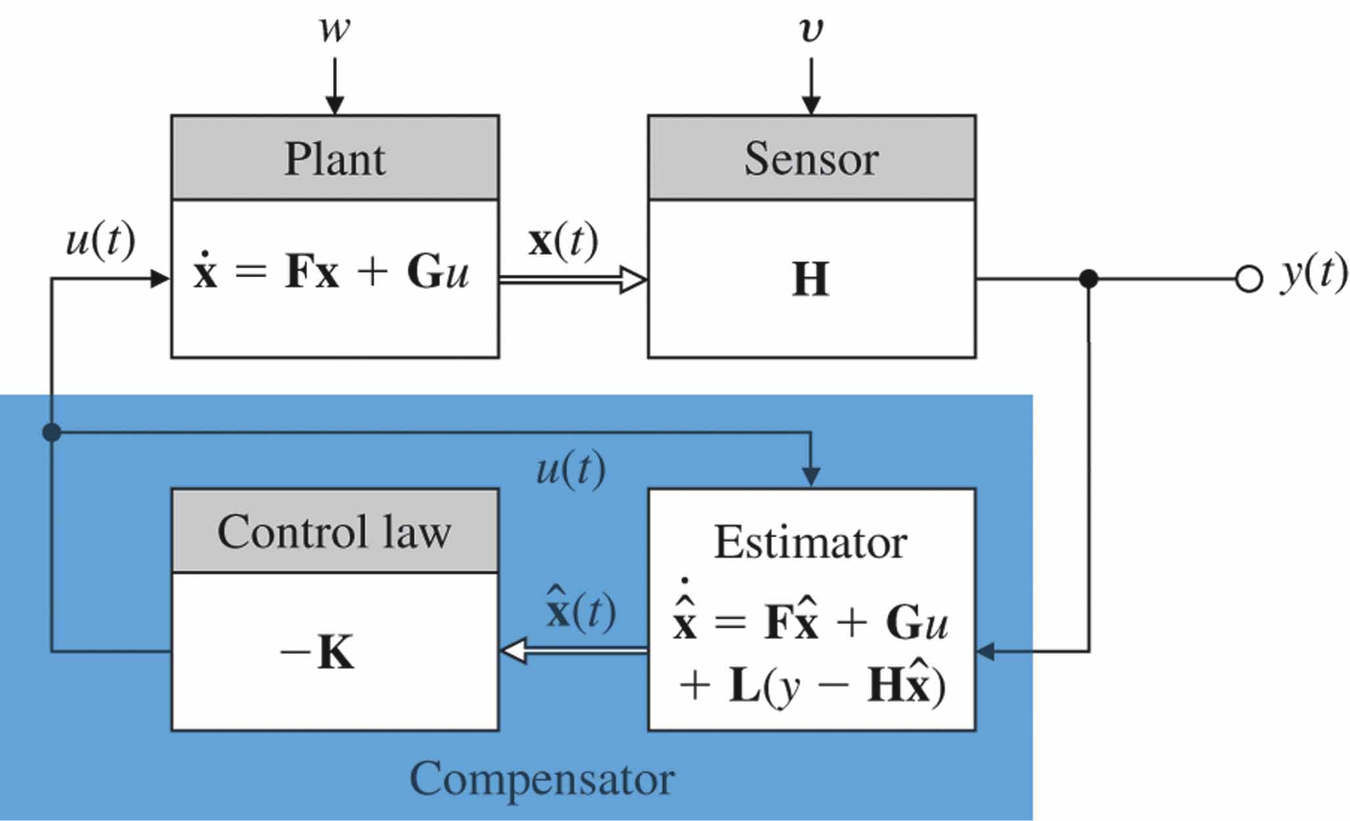
\includegraphics[width=0.7\linewidth]{content/img/kompensator}
\caption{}
\label{fig:kompensator}
\end{figure}
Übertragungsfunktion lässt sich berechnen durch:
\begin{align*}
    &D(s) = \frac{U(s)}{Y(s)}\\
    &U(s) = \det(P(s)) = \det\left[\begin{array}{l|r}
    s\bs{I}- \bs{A} & \bs{L}\\\hline
    \bs{K} & 0
    \end{array}\right]\\
    &Y(s) = \det(s\bs{I}-\bs{F}+\bs{LH}+\bs{GK})
\end{align*} 

\end{tcolorbox}


    \setcounter{section}{14}
\section{Optimale Regelung}
\begin{tcolorbox}[colback=white!10!white,
                  colframe=blue!50!black,
                  title=Definitheit einer symmetrischen (Tuning-) Matrix]
    \begin{minipage}{0.3\textwidth}
        \centering
        $\begin{bmatrix}a & b \\ b & c\end{bmatrix}$
    \end{minipage}
    \begin{minipage}{0.65\textwidth}
        \centering
        \begin{table}[H]
        \centering
        \tablestyle
        \begin{tabular}{lccc}
            \tableheadcolor
                \tablehead Matrix &
                \tablehead $a$ &
                \tablehead $c$ &
                \tablehead $a \cdot c$ \\
            \tablebody
            positiv definit $(\succ 0)$       & $  > 0$ & -       & $  > b^2$\\
            positiv semidefinit $(\succeq 0)$ & $\ge 0$ & $\ge 0$ & $\ge b^2$\\
            \tableend\tablebody
            negativ definit $(\prec 0)$       & $  < 0$ & -       & $  > b^2$\\
            negativ semidefinit $(\preceq 0)$ & $\le 0$ & $\le 0$ & $\ge b^2$\\
            \tableend\tablebody
            indefinit                         & -       & -       & $  < b^2$\\
            \tableend
        \end{tabular}
    \end{table}
    \end{minipage}
\end{tcolorbox}

\subsection{LQ-Regler - optimaler Regler}
\begin{tcolorbox}[colback=white!10!white,colframe=green!30!black] 
    \textbf{Anforderung an Tuning-Matrizen:}
    \begin{align*}
        \bs{P} = \bs{P}^T \succeq 0
        && \bs{Q} = \bs{Q}^T \succeq 0
        && \bs{R} = \bs{R}^T \succ 0
    \end{align*}
    
    \tcblower
    \begin{enumerate}
        \item Löse Gleichung
            \begin{align*}
                \bs{0} = -\bs{F}^T\bs{P} - \bs{PF}
                - \bs{PG}\bs{R}^{-1}\bs{G}^T\bs{P} - \bs{Q}
            \end{align*}
        \item optimaler Regeleingang
        \begin{align*}
            u(t) = - \bs{Kx}(t) = -(\underbrace{\bs{R}^{-1}\bs{G}^T\bs{P}}_{K})\bs{x}(t)
        \end{align*}
        \item Eine Lösung ist gegeben, wenn alle instabilen Zustände steuerbar sind  -\textbf{stabilisierbar}
        \item Instabile Moden müssen durch die Kostenfunktion erfasst werden
        \item Stabil, wenn das System \begin{align*}
            \dot{\bs{x}} = \bs{Fx} && \bs{y} = \bs{Q}^{\frac{1}{2}}\bs{x} 
        \end{align*}
        \textbf{detektierbar} ist. Alle instabilen Zustände sind beobachtbar.
        \item Wenn $[\bs{H},\bs{F}]$ detektierbar ist typischerweise $Q = \bs{H}^T\bs{H}$ 
    \end{enumerate}

\begin{tcolorbox}[colback=white!10!white,colframe=gray!30!black] 
    Stabilisierbarkeit lässt sich durch die B-Matrix, Detektierbarkeit durch die C-Matrix erkennen, wenn das System in Modalform vorliegt.
\end{tcolorbox}    
\begin{tcolorbox}[colback=white!10!white,colframe=gray!30!black] 
    Ein Maß für die Güte eines Reglers ist die Kostenfunktion $J$. Die Funktion spiegelt die Kosten  für einen Regler wider. Man minimiert die Kostenfunktion. $\Rightarrow$ Ricatti-Gleichung
    \begin{align*}
        J = \int_{0}^{\infty}(\bs{x}^T(t)\bs{Qx}(t)+\bs{u}^T(t)\bs{Ru}(t))dt
    \end{align*}
\end{tcolorbox}
\end{tcolorbox}


    \setcounter{section}{15}
\section{Kalman-Filter - optimaler Schätzer}
\begin{tcolorbox}[colback=white!10!white,colframe=green!30!black] 
    \textbf{Das zeitinvariante Kalman-Filter} ist realisierbar, wenn
    $(\bs{H},\bs{F})$ - detektierbar und $(\bs{F},\bs{Q}^{\frac{1}{2}})$ stabilisierbar. Die Lösung der Matrix-Ricatti Gleichung ist dann ein \textbf{positiv-semidefinite konstante} Matrix $\bs{P}$. 
    \begin{tcolorbox}[colback=white!10!white,colframe=green!30!black]
        \begin{align*}
        &    (\bs{H},\bs{F})& &\dot{\bs{x}} = \bs{Fx} & &\bs{y} = \bs{Hx}\\
        &    (\bs{F},\bs{Q}^{\frac{1}{2}})&& \dot{\bs{x}} = \bs{Fx}+\bs{Q}^{\frac{1}{2}}u & &
        \end{align*}
    \end{tcolorbox}
    
    Für die Matrizen gilt: $\bs{Q}\succeq0$ - semidefinit und $\bs{R}\succ0$ - definit. (manchmal werden diagonale Matrizen angenommen.)
    \\\\
    \textit{Bemerkung:} Für eine einfache Lösung müssen Rauschprozesse \textbf{Prozessrauschen $w(t)$} und \textbf{Messrauschen $v(t)$} weiß und unkorreliert sein. $E(w(t))= E(v(t)) =0$ und $E(w(t),v(t)^T)=0$
    Kovarianz kann folgendermaßen ermittelt werden:
        \begin{align*}
            w(t) & & E(w(t)w(t)^T) =\bs{Q}\delta(t-\tau) && \bs{Q} \succeq 0 \\ v(t) & & E(v(t)v(t)^T) = \bs{R}\delta(t-\tau) && \bs{R} \succ 0
         \end{align*}
    
    \tcblower
    \textbf{Vorgehensweise:}
    \begin{enumerate}
        \item Löse die Gleichung\begin{align*}
            \bs{0} = \bs{FP} + (\bs{FP})^T -(\bs{HP})^T\bs{R}^{-1}\bs{HP} +\bs{Q}
        \end{align*}
        \item Für $2\times2$-Matrizen wird ein symmetrisches $\bs{P}$ angenommen\begin{align*}
            \begin{bmatrix}
            p_1 & p_2 \\ p_2 & p_3
            \end{bmatrix}
        \end{align*}
            \item Ein LGS mit drei Unbekannten $p_1,p_2,p_3$ lösen 
            \item Nur die Lösung mit $p_i\geq 0$   $\forall i$ wählen
            \item Setze $\bs{P}$ in die Gleichung ein für konstante Rückführmatrix
             \begin{align*}
                \bs{L} = \bs{PH}^T\bs{R}^{-1}
            \end{align*} 
    \end{enumerate}
    
    
\end{tcolorbox}

    \setcounter{section}{16}
\section{Diskrete Systeme}
\begin{tcolorbox}[colback=white!10!white,
                  colframe=green!30!black,
                  title=Zusammenhang $s$ und $z$]
\textbf{Abbildung:}

Linke komplexe s-Halbebene $\Longrightarrow$ Einheitskreis $|z|=1$

$z = e^{sT}$ ist die Abbildungsvorschrift
\end{tcolorbox}

\begin{tcolorbox}[colback=white!10!white,
                  colframe=green!30!black,
                  title=$z$-Übertragungsfunktion]
    \begin{align*}
        \mathcal{Z}\{ f(k-n)\} = z^{-n}F(z)
    \end{align*}
    Allgemeine DGL (2. Ordnung):
    \begin{align*}
        &y(k)    = -a_1y(k-1)-a_2(k-2)+b_0u(k)\\&+b_1u(k-1)+b_2u(k-2)\\
        &\mathcal{Z}\{ y(k)\}  = Y(z)\\
        &Y(z) = (-a_1z^{-1}-a_2z^{-2})Y(z) 
        +(b_0+b_1z^{-1}+b_2z^{-2})U(z)\\
        &\frac{Y(z)}{U(z)} = \frac{b_0+b_1z^{-1}+b_2z^{-2}}{1+a_1z^{-1}+a_2z^{-2}}
    \end{align*}
    \textbf{Ablesen des Pols:}
    \begin{align*}
        & Y(z) = \frac{1}{1-\alpha z^-1} &\Rightarrow z_1 = \alpha
    \end{align*}
    \begin{tcolorbox}[colback=white!10!white,colframe=green!30!black]
        \textbf{Endwertsatz der $z$-Transformation:}
        
        Kontinuierliches System:
        \begin{align*}
            \lim\limits_{t\to\infty} x(t) = x_{\text{stat}} = \lim\limits_{s\to 0 }sX(s)
        \end{align*}
        Diskretes System:
        \begin{align*}
             \lim\limits_{k\to\infty} x(k) =  x_{\text{stat}} = \lim\limits_{z\to 1 }X(z)
        \end{align*}
    \end{tcolorbox}
\end{tcolorbox}

\begin{tcolorbox}[colback=white!10!white,
                  colframe=blue!30!black,
                  title=$z$-Übertragungsfunktion: Halteglied und kontinuierliches System in Reihe]
    Das ist eine Approximation über Reihenschaltung Halteglied und kontinuierliches System:
    \begin{align*}
        G(z) &= \frac{z-1}{z}\mathcal{Z}\left\{\frac{G(s)}{s}\right\}
    \end{align*}
\end{tcolorbox}

\begin{tcolorbox}[colback=white!10!white,
                  colframe=blue!30!black,
                  title=Reglerentwurf - diskrete Äquivalente]
    \textbf{Vorgehen:}
    \begin{enumerate}
        \item Entwerfe kontinuierlichen Regler
        \item Diskretisiere den Regler
        \item Bestätige Entwurf durch diskrete Analyse
    \end{enumerate}
    Genügt eine lineare Interpolation kann die \textbf{Trapezregel} 
    (Substitution) zur \textbf{Diskretisierung} verwendet werden:
    \begin{align*}
        s &= \frac{2}{T} \cdot \frac{1-z^{-1}}{1+z^{-1}}
    \end{align*}
\end{tcolorbox}
    \setcounter{section}{17}
\section{Diskrete Fundamentalmatrix}
\begin{tcolorbox}[colback=white!10!white,colframe=green!30!black,title=Definition] 
    \begin{align*}
        \bs{A}_d(T)= e^{\bs{A}T} && B_d = \int_{0}^{T}\bs{A}_d
        (\tau)d\tau    \cdot \bs{B} 
    \end{align*}
    Mit Taylorzerlegung kann man $A_d$ berechnen:
    \begin{align*}
        e^{\bs{A}t}  &= \bs{I} + \bs{A}t+\bs{A}^2\frac{t^2}{2!} + \bs{A}^3\frac{t^3}{3!}+ \ldots\\
        \frac{d}{dt}e^{\bs{A}t} &= \bs{A} + \bs{A}^2t+\bs{A}^3\frac{t^2}{2!} + \ldots
    \end{align*}
\end{tcolorbox}
\begin{tcolorbox}[colback=white!10!white,colframe=blue!30!black,title=KOCHREZEPT: Fundamentalmatrix Berechnung] 
    \begin{align*}
        \bs{A}_d(T) &= \mathcal{L}^{-1}\{(s\bs{I}-\bs{A})^{-1}\}\\
        \bs{B}_d(T) &= \mathcal{L}^{-1}\{(\frac{1}{s}\bs{A}_d(s)\cdot \bs{B})\}
    \end{align*}
    Für $2\times2$-Matrix lässt sich $A_d$ so bestimmen:
    \begin{align*}
        \bs{A}_d(s) &= \frac{1}{|s\bs{I}-\bs{A}|} adj(s\bs{I}-\bs{A})\\
        \bs{A}_d(T) &= \mathcal{L}^{-1}\{A_d(s)\}
    \end{align*}
    \tcblower
    \begin{align*}
        \mathcal{C}_d &= \begin{bmatrix}
        \bs{B}_d & \bs{A}_d\bs{B}_d & \ldots & \bs{A}_d^{n-1}\bs{B}_d
        \end{bmatrix}\\
        \mathcal{O}_d &= \begin{bmatrix}
        \bs{C} \\\bs{C}\bs{A}_d \\ \vdots \\ \bs{C}\bs{A}_d^{n-1}
        \end{bmatrix}
    \end{align*}
    \begin{tcolorbox}[colback=white!10!white,
                      colframe=gray!70!black,
                      title=Steuerbarkeit und Beobachtbarkeit]
        Das zeitdiskrete System ($\bs{A}_d,\bs{B}_d$) ist vollständig 
        \textbf{steuerbar} bzw. \textbf{beobachtbar}, wenn kontinuierliches 
        System ($\bs{A},\bs{B}$) es ist und wenn die Abtastzeit folgendes erfüllt:
        \begin{align*}
            T < \frac{\pi}{\omega_{j,\text{max}}}
        \end{align*}
        $\omega_{j,\text{max}}$ ist betraglich größter Eigenwert von $A$
    \end{tcolorbox}
\end{tcolorbox}

\end{multicols}
\end{document}
